% genesis_mnras.tex
%
% GENESIS — MNRAS Manuscript
% Based on mnras_template.tex v3.3 (April 2024)
%
% FILL MARKERS:  \FILL{description}  — replace with actual values
% TODO MARKERS:  % TODO: ...         — action items before submission
%
% Compile:  pdflatex genesis_mnras.tex
%           bibtex   genesis_mnras
%           pdflatex genesis_mnras.tex (x2)

%%%%%%%%%%%%%%%%%%%%%%%%%%%%%%%%%%%%%%%%%%%%%%%%%%
\documentclass[usenatbib]{mnras}

% \usepackage{newtxtext,newtxmath}  % preferred; uncomment if available
\usepackage{mathptmx}  % fallback Times font
\usepackage[T1]{fontenc}

\DeclareRobustCommand{\VAN}[3]{#2}
\let\VANthebibliography\thebibliography
\def\thebibliography{\DeclareRobustCommand{\VAN}[3]{##3}\VANthebibliography}

%%%%% EXTRA PACKAGES %%%%%
\usepackage{graphicx}
\graphicspath{{figs/lh/}{figs/cv/}}
\usepackage{amsmath}
\usepackage{amssymb}
\usepackage{booktabs}
\usepackage{xcolor}
\usepackage{microtype}
\usepackage{afterpage}
\usepackage{placeins}
\usepackage{float}
\usepackage{multirow}
% \usepackage{siunitx}  % commented out for compilation (not used in body)
\usepackage{enumitem}
\hypersetup{hypertexnames=false}

%%%%% CUSTOM COMMANDS %%%%%
\newcommand{\FILL}[1]{\textcolor{red}{\textbf{[#1]}}}
\newcommand{\Mcdm}{M_{\rm cdm}}
\newcommand{\Mgas}{M_{\rm gas}}
\newcommand{\Tgas}{T}
\newcommand{\Om}{\Omega_{\rm m}}
\newcommand{\sig}{\sigma_8}
\newcommand{\thetavec}{\boldsymbol{\theta}}
\newcommand{\kvec}{\boldsymbol{k}}
\newcommand{\Pk}{P(k)}
\newcommand{\Pkab}{P_{ab}(k)}
\newcommand{\rab}{r_{ab}(k)}
\newcommand{\DeltaP}{\Delta P/P}
\newcommand{\figfull}{0.86\textwidth}
\newcommand{\figwide}{0.86\textwidth}
\newcommand{\figpair}{0.44\textwidth}
\newcommand{\figtriple}{0.32\textwidth}
\newcommand{\figcol}{\columnwidth}
\newcommand{\figcolwide}{\columnwidth}
\newcommand{\figcolsquare}{0.70\columnwidth}
% \FloatBarrier is provided by placeins package
\newcommand{\figplaceholder}[3]{%
  \fbox{%
    \begin{minipage}[c][#2][c]{#1}
      \centering
      \vspace{0pt}
      \textbf{Figure Placeholder}\\[0.35em]
      {\footnotesize #3}
    \end{minipage}%
  }%
}
\newcommand{\layoutplaceholder}[3]{%
  \begingroup
  \setlength{\fboxsep}{0pt}%
  \fbox{%
    \begin{minipage}[c][#2][c]{#1}
      \centering
      \footnotesize
      \textbf{#3}\\[0.35em]
      {\scriptsize placeholder}
    \end{minipage}%
  }%
  \endgroup
}
\newenvironment{inlinefigure}[1]{%
  \par\smallskip
  \refstepcounter{figure}\label{#1}%
  \noindent\begin{minipage}{\columnwidth}
  \centering
}{%
  \end{minipage}%
  \par\smallskip
}
\newcommand{\inlinefigcaption}[1]{%
  \par\vspace{0.4ex}%
  {\footnotesize\textbf{Figure~\thefigure.} #1\par}%
}

\setcounter{topnumber}{3}
\setcounter{dbltopnumber}{3}
\renewcommand{\topfraction}{0.92}
\renewcommand{\dbltopfraction}{0.92}
\renewcommand{\textfraction}{0.08}
\renewcommand{\floatpagefraction}{0.86}
\renewcommand{\dblfloatpagefraction}{0.86}
\setlength{\textfloatsep}{7pt plus 2pt minus 2pt}
\setlength{\dbltextfloatsep}{7pt plus 2pt minus 2pt}
\setlength{\floatsep}{6pt plus 2pt minus 2pt}
\setlength{\dblfloatsep}{6pt plus 2pt minus 2pt}

%%%%%%%%%%%%%%%%%%% TITLE PAGE %%%%%%%%%%%%%%%%%%%

\title[GENESIS: Flow-Based Cosmological Emulator]{
GENESIS: Generative Emulation of Cosmological Multifield Maps with
Optimal-Transport Flow Matching
}

\author[M. Park]{%
Minje Park$^{1}$\thanks{E-mail: Pmj032400@naver.com}
\\
$^{1}$Department of Physics, Sungkyunkwan University, Suwon 16419, Republic of Korea
}

\date{Accepted XXX. Received YYY; in original form ZZZ}

%\pubyear{\the\year{}}

%%%%%%%%%%%%%%%%%%%%%%%%%%%%%%%%%%%%%%%%%%%%%%%%%%

\begin{document}
%\label{firstpage}
%\pagerange{\pageref{firstpage}--\pageref{lastpage}}
\maketitle
\makeatletter
\gdef\@journal{\makebox[\textwidth]{\hfill Preprint \tod@y\hfill
  Compiled using MNRAS \LaTeX\ style file v\@version}}
\def\ps@titlepage{\let\@mkboth\@gobbletwo
 \def\@oddhead{\footnotesize\@journal}
 \def\@oddfoot{}
 \def\@evenhead{\footnotesize\@journal\hfill}
 \def\@evenfoot{}
 \def\sectionmark##1{}
 \def\subsectionmark##1{}}
\thispagestyle{titlepage}
\def\ps@headings{\let\@mkboth\markboth
 \def\@oddhead{\Large\hfill{\it\@shorttitle}\hspace{1.5em}%
   \rm\@ddell\thepage}
 \def\@oddfoot{}
 \def\@evenhead{\Large\@ddell\thepage\hspace{1.5em}\it\@shortauthor\hfill}
 \def\@evenfoot{}
 \def\sectionmark##1{\markboth{##1}{}}
 \def\subsectionmark##1{\markright{##1}}}
\def\ps@myheadings{\let\@mkboth\@gobbletwo
 \def\@oddhead{\Large\hfill\it\rightmark\hspace{1.5em}\rm\@ddell\thepage}
 \def\@oddfoot{}
 \def\@evenhead{\Large\@ddell\thepage\hspace{1.5em}\it\leftmark\hfill}
 \def\@evenfoot{}
 \def\sectionmark##1{}
 \def\subsectionmark##1{}}
\ps@headings
\makeatother

%% ── Abstract ──────────────────────────────────────────────────────────────
% \begin{abstract}
% Diffusion models have accelerated the development of generative
% modelling across many domains and have been widely adopted in
% cosmology for field generation, emulation, and parameter inference.
% However, diffusion-based approaches typically require many sampling
% steps and generally provide likelihood information only through a
% lower bound. Flow matching has recently emerged as an alternative
% generative framework with stable training, efficient sampling, and
% tractable likelihood evaluation, but its use in cosmology remains
% limited.

% We present \textsc{Genesis}, a conditional generative emulator for
% multifield cosmological maps based on optimal-transport flow
% matching. To our knowledge, this is the first application of
% optimal-transport flow matching to conditional multifield generation
% with CAMELS/CMD maps. The model jointly generates dark matter density,
% gas density, and gas temperature maps, conditioned on the two
% cosmological parameters $(\Om,\sig)$ and four astrophysical feedback
% parameters of CAMELS. Across held-out parameter-varying and
% fixed-parameter tests, \textsc{Genesis} produces multifield samples
% that broadly reproduce the target CAMELS statistics and preserve the
% main correlations among the three fields. Sampling is also practical:
% in the current implementation, generating one multifield map triplet
% takes about six seconds on an NVIDIA A100 GPU.

% As an initial demonstration of the likelihood capability of the
% learned flow, we perform a two-dimensional $\Om$--$\sig$ scan for one
% CAMELS map while fixing the remaining parameters, and find that the
% relative likelihood peaks at the input parameter values within the
% evaluated grid. These results indicate that optimal-transport flow
% matching is a promising framework for fast conditional multifield
% cosmological emulation, with potential for field-level
% likelihood-based inference.
% \end{abstract}
\begin{abstract}
Diffusion models have accelerated the development of generative
modelling across many domains and have been widely adopted in
cosmology for field generation, emulation, and parameter inference.
However, diffusion-based approaches typically require many sampling
steps and generally provide likelihood information only through a
lower bound. Flow matching has recently emerged as an alternative
generative framework with stable training, efficient sampling, and
tractable likelihood evaluation, but its use in cosmology remains
limited. We present \textsc{Genesis}, a conditional generative
emulator for multifield cosmological maps based on optimal-transport
flow matching. To our knowledge, this is the first application of
optimal-transport flow matching to conditional multifield generation
with CAMELS/CMD maps. The model jointly generates dark matter
density, gas density, and gas temperature maps, conditioned on the two
cosmological parameters $(\Omega_{\rm m},\sigma_8)$ and four
astrophysical feedback parameters of CAMELS. Across held-out
parameter-varying and fixed-parameter tests, \textsc{Genesis}
produces multifield samples that broadly reproduce the target CAMELS
statistics and preserve the main correlations among the three fields.
Sampling is also practical: in the current implementation, generating
one multifield map triplet takes about six seconds on an NVIDIA A100
GPU. As an initial demonstration of the likelihood capability of the
learned flow, we perform a two-dimensional $\Omega_{\rm m}$--$\sigma_8$
scan for one CAMELS map while fixing the remaining parameters, and
find that the relative likelihood peaks at the input parameter values
within the evaluated grid. These results indicate that
optimal-transport flow matching is a promising framework for fast
conditional multifield cosmological emulation, with potential for
field-level likelihood-based inference.
\end{abstract}

\begin{keywords}
Cosmological fields ---
Cosmological parameters ---
Generative models ---
Parameter inference ---
Neural networks
\end{keywords}

%%%%%%%%%%%%%%%%%%%%%%%%%%%%%%%%%%%%%%%%%%%%%%%%%%

%%%%%%%%%%%%%%%%% BODY OF PAPER %%%%%%%%%%%%%%%%%%

%% =============================================================
%%  §1  INTRODUCTION
%% =============================================================
\section{Introduction}
\label{sec:intro}
In modern cosmology, machine learning has emerged as an indispensable
tool across a broad range of problems,
including cosmological parameter inference
\citep{Ravanbakhsh2017,Cranmer2020}, field-level analyses and baryonic
field mapping \citep{JoKim2019,Zhang2019}, and generative modelling
and emulation of cosmological fields
\citep{Mustafa2019,He2019,Perraudin2021}.
As in many other machine-learning domains, progress in these problems
depends on access to large and diverse data sets. In cosmology, however,
such data sets are often provided by cosmological hydrodynamic
simulations that model complex baryonic physics, making them
computationally expensive to produce.
The Cosmology and Astrophysics with Machine Learning Simulations
\citep[CAMELS;][]{Villaescusa2021} project was conceived to address
this challenge by providing thousands of simulations in which both
cosmological and astrophysical parameters are varied in a controlled
fashion. As part of the CAMELS project, the CAMELS Multifield Dataset \citep[CMD;][]{Villaescusa2022}
releases these simulations as 2D maps and 3D grids of multiple
physical fields, including dark matter density, gas density, and gas temperature, 
together with their associated simulation parameters.
Since these fields are co-registered and share the same underlying
CAMELS parameters, CMD provides a natural testbed for studying not
only individual field statistics but also correlations among
physically related observables.

Meanwhile, in the machine-learning domain, deep generative models
have made substantial progress over the past decade. This progress
can be viewed as a sequence of advances in which successive model
families addressed key limitations of earlier approaches while
introducing new trade-offs. The variational autoencoder \citep[VAE;][]{Kingma2014} 
provided an early foundation by learning structured latent representations of
data, although it often produced overly smooth samples. Generative adversarial networks
\citep[GANs;][]{Goodfellow2014} shifted the focus toward perceptual
sample quality by training a generator and a discriminator in an
adversarial game, yielding sharper samples but
remaining vulnerable to mode collapse. Normalizing flows \citep{RezendeMohamed2015}
provided exact likelihood evaluation through invertible mappings
between a simple prior and the data distribution, but their
architectural constraints often limited their expressiveness.
More recently, diffusion models \citep{Ho2020,Song2021} have reshaped the generative modelling 
landscape by providing a stable and scalable approach to learning complex data
distributions through the reversal of a gradual noising process. 
However, diffusion models are subject to two key limitations: 
their training objective is tied to an evidence lower bound of the likelihood (ELBO), 
making exact likelihood evaluation intractable, and sampling typically requires many steps.
Flow matching \citep{Lipman2023} has recently emerged as an
alternative that mitigates both limitations. It trains a
neural network to approximate the time-dependent velocity field that
transports a simple prior distribution into the data distribution,
modelling the evolution of the probability path over time. Through
its connection to continuous normalizing flows \citep{Chen2018}, this
formulation supports likelihood evaluation via the
change-of-variables formula. Furthermore, when combined with
optimal-transport couplings \citep{Lipman2023}, flow matching induces
straighter probability paths between the two distributions, reducing
the number of steps required for sampling.

This methodological progression has also shaped the use of generative
models in cosmology. Early approaches applied GANs and normalizing
flows to cosmological multifield emulation, HI-map generation, and
likelihood-based inference
\citep{Andrianomena2022,Andrianomena2024,Hassan2021HIFlow,Friedman2022HIGlow}.
Diffusion models were subsequently adopted for dark-matter
reconstruction from biased tracers
\citep{Park2023Diffusion,Ono2024Debiasing}, HI-map emulation
\citep{Hassan2023HIDM}, and dark matter density-field generation and
parameter inference \citep{Mudur2024,Mudur2024DiffHMC}. More recent
work has explored latent-diffusion upscaling of cosmological fields
\citep{Mishra2026} and stochastic-interpolant baryonic field mapping
\citep{Horowitz2025}. Flow matching has also begun to enter cosmology, for example in
\citet{Kannan2025}, which uses flow matching for scale-aware
representation learning of field-level cold dark matter simulations.
However, direct conditional generation and emulation of multiple
co-registered cosmological fields remains largely unexplored.

This motivates our central objective: to bring optimal-transport flow
matching (OT-FM) to direct conditional cosmological field generation
and emulation, thereby exploiting key advantages of OT-FM that remain
largely unused in cosmological field modelling, including efficient
sampling through straighter transport paths and likelihood evaluation
within the continuous normalizing flow (CNF) framework \citep{Chen2018}.
In addition to statistical fidelity, we report the practical sampling
cost of the trained model: in the current implementation, generating
200 independent multifield map triplets at a fixed conditioning vector
takes roughly 20 minutes on a single NVIDIA A100 GPU.
Beyond the choice of generative framework, existing generative models
built on CAMELS/CMD data have typically used only part of the available
conditioning information, focusing primarily on the two cosmological
parameters ($\Om$, $\sig$)
\citep{Andrianomena2022,Andrianomena2024,Mudur2022DDPM,Hassan2023HIDM,Mudur2024,Mudur2024DiffHMC}.
The four astrophysical feedback parameters varied in CAMELS
($A_{\rm SN1}$, $A_{\rm SN2}$, $A_{\rm AGN1}$, $A_{\rm AGN2}$) have
therefore generally been fixed, ignored, or marginalized over, despite
their strong influence on baryonic fields. At the same time, most
existing generative models have targeted individual fields in isolation
\citep{Hassan2021HIFlow,Mudur2022DDPM,Hassan2023HIDM,Mudur2024}.
Together, these limitations point to the need for a fully conditioned
multifield generative emulator that can model correlations among
physically coupled fields.

In this work, we introduce \textsc{Genesis}
(\textbf{GEN}erative \textbf{E}mulator for
\textbf{S}imulation and parameter \textbf{I}nference from cosmological field\textbf{s}),
a conditional continuous normalizing flow trained with OT-FM for
multifield cosmological emulation and field-level likelihood-based
parameter inference. Our contributions are as follows.
\begin{enumerate}[label=\arabic*., leftmargin=*, labelsep=0.5em]
  \item To the best of our knowledge, \textsc{Genesis} is the first
        generative model to apply OT-FM to direct conditional
        generation of multifield cosmological maps.
        While GAN-based models have previously generated multiple
        cosmological fields \citep{Andrianomena2022,Andrianomena2024},
        no prior work has produced $\Mcdm$,
        $\Mgas$, and $\Tgas$ jointly.

  \item \textsc{Genesis} conditions on the full six-dimensional
        CAMELS parameter vector associated with each CMD map, namely
        the two cosmological parameters ($\Om$, $\sig$) and the four
        astrophysical feedback parameters
        ($A_{\rm SN1}$, $A_{\rm SN2}$, $A_{\rm AGN1}$, $A_{\rm AGN2}$).
        This conditioning enables the model to capture the distinct
        responses of dark matter density, gas density, and gas
        temperature to cosmological and feedback variations across the
        CAMELS design space. To the best of our knowledge, this is the
        first generative model to produce multifield maps conditioned 
        on this full parameter vector.

  \item We illustrate the potential of \textsc{Genesis} for
        field-level likelihood-based parameter inference without any
        additional training. Through the CNF change-of-variables
        formula, the model assigns likelihoods to input multifield maps
        under candidate conditioning vectors. As a proof of concept,
        we fix one held-out CMD multifield map $\mathbf{x}_1$ and scan
        the $(\Om,\sig)$ plane while holding the four astrophysical
        feedback parameters at their true values. Within the evaluated
        grid, the maximum-likelihood point coincides with the true
        CAMELS parameter point, $(\Om,\sig)=(0.3054,0.8090)$, and the
        Wilks-theorem 1$\sigma$ contour encloses neighbouring grid
        points. We therefore frame this as evidence that the likelihood
        surface is centred on the truth at the scan resolution, rather
        than as a unique parameter resolution within stochastic noise.
\end{enumerate}

The remainder of this paper is organized as follows.
Section~\ref{sec:data} describes the CAMELS simulations, the CMD
field data, and our field choices.
Section~\ref{sec:methods} presents the OT-FM framework and \textsc{Genesis}
architecture.
Sections~\ref{sec:eval} and~\ref{sec:cv_eval} evaluate \textsc{Genesis}
on a test split of the CAMELS/CMD Latin-hypercube set and on an
independent constant-parameter set, respectively.
Section~\ref{sec:likelihood_inference} presents a likelihood scan as a proof of
concept, demonstrating the potential of \textsc{Genesis} for field-level
parameter inference.
Section~\ref{sec:discussion} discusses the architectural design choices,
proximity to the cosmic variance floor, comparison with prior work, and identifies
limitations and future directions. Section~\ref{sec:conclusions} concludes.

%% =============================================================
%%  §2  DATA
%% =============================================================
\section{CAMELS Multifield Dataset}
\label{sec:data}
This section describes the publicly released 2D maps from the CAMELS
Multifield Dataset (CMD) used by \textsc{Genesis}
(Section~\ref{sec:camels}), the three target channels
($\Mcdm$, $\Mgas$, and $\Tgas$) and the IllustrisTNG data splits
adopted in this work (Section~\ref{sec:fields}), and the six
conditioning parameters and their field-level sensitivities
(Section~\ref{sec:params}).

\subsection{IllustrisTNG 2D maps}
\label{sec:camels}
We use the IllustrisTNG 2D maps from the CMD
\citep{Villaescusa2022}, whose hydrodynamic runs adopt the baryonic
model of \citet{Weinberger2017} and \citet{Pillepich2018IllustrisTNG}.
These simulations evolve a periodic box of side
$25\,h^{-1}$~Mpc with $256^3$ dark matter particles and an equal
number of initial gas cells from $z=127$ to $z=0$.
Within the public IllustrisTNG map release, we use the LH set for
training, validation, and testing, and the CV set to assess
statistical consistency across independent realizations at fixed
parameter values. For each simulation and target channel, the release
provides 15 projected two-dimensional maps, obtained from five
non-overlapping slices along each of the three Cartesian axes.

\begin{description}[font=\normalfont\bfseries,leftmargin=2.2em,labelsep=0.6em]
  \item[LH set.] One thousand simulations sampling the
        six-dimensional CAMELS parameter space with a Latin-hypercube
        design (see Table~\ref{tab:params} for parameter ranges).
        We use this parameter-varying set for training, validation,
        and testing, partitioning it into 800 training, 100
        validation, and 100 test simulations.
  \item[CV set.] Twenty-seven simulations at the fiducial parameter
        vector $(\Om, \sig, A_{\rm SN1}, A_{\rm SN2}, A_{\rm AGN1},
        A_{\rm AGN2}) = (0.30, 0.80, 1, 1, 1, 1)$, differing only
        in their initial conditions. We use this set to test whether
        generated samples are statistically consistent with
        independent simulations at the same parameter point.
\end{description}

\subsection{Field definitions}
\label{sec:fields}

We select three CMD fields as the joint emulation target of
\textsc{Genesis}: projected dark matter surface mass density
($\Mcdm$), projected gas surface mass density ($\Mgas$), and projected
mass-weighted gas temperature ($\Tgas$). Each map comprises
$256\times256$ pixels covering a field of view of
$(25\,h^{-1}\,\mathrm{Mpc})^2$, extracted from the $z=0$ snapshot, and
is constructed by projecting particle properties onto a regular grid
using an adaptive smoothing kernel \citep{Villaescusa2022}.

Together, these three fields encode the dominant matter components and
the thermodynamic state of the gas. Their cross-correlations provide
sensitive diagnostics of baryonic feedback, motivating the joint
emulation approach of \textsc{Genesis}.

\subsection{Conditioning parameters and field-level sensitivity}
\label{sec:params}

\textsc{Genesis} is conditioned on the full six-dimensional CAMELS
parameter vector
\begin{equation}
  \boldsymbol{\theta} =
  (\Om,\,\sig,\,A_{\rm SN1},\,A_{\rm SN2},\,A_{\rm AGN1},\,A_{\rm AGN2}),
  \label{eq:theta}
\end{equation}
which characterizes each IllustrisTNG simulation in CMD
\citep{Villaescusa2021,Villaescusa2022}.
Table~\ref{tab:params} summarizes the Latin-hypercube ranges and
physical meaning of each parameter.

\begin{table}
  \centering
  \small
  \setlength{\tabcolsep}{4pt}
  \renewcommand{\arraystretch}{1.08}
  \begin{tabular*}{\columnwidth}{@{\extracolsep{\fill}}lll@{}}
    \toprule
    Parameter & LH range & Physical meaning \\
    \midrule
    $\Om$          & $[0.1,\;0.5]$  & Total matter density fraction \\
    $\sig$         & $[0.6,\;1.0]$  & Linear fluctuation amplitude \\
    $A_{\rm SN1}$  & $[0.25,\;4.0]$ & SN wind energy per SFR \\
    $A_{\rm SN2}$  & $[0.5,\;2.0]$  & SN wind speed \\
    $A_{\rm AGN1}$ & $[0.25,\;4.0]$ & AGN energy per BH accretion rate \\
    $A_{\rm AGN2}$ & $[0.5,\;2.0]$  & AGN kinetic ejection speed \\
    \bottomrule
  \end{tabular*}
  \caption{CAMELS IllustrisTNG conditioning parameters, their
    Latin-hypercube ranges, and physical interpretations
    \citep{Villaescusa2021,Villaescusa2022}.}
  \label{tab:params}
\end{table}

The two \emph{cosmological parameters} govern the overall amplitude
and shape of the matter power spectrum.
$\Om$ sets the total matter density of the Universe, while
$\sig$ defines the root-mean-square amplitude of linear density
fluctuations smoothed on $8\,h^{-1}$~Mpc scales.
Both parameters primarily govern dark matter clustering, with the
baryonic fields responding through the evolving gravitational
potential.
The four \emph{astrophysical feedback parameters} encode the
subgrid prescriptions of the IllustrisTNG model
\citep{Weinberger2017,Pillepich2018IllustrisTNG}.
$A_{\rm SN1}$ and $A_{\rm SN2}$ control two properties of
supernova-driven galactic winds: the energy emitted per unit
star-formation rate and the wind speed, respectively.
$A_{\rm AGN1}$ and $A_{\rm AGN2}$ represent the energy released per
unit black hole accretion rate and the ejection speed of the kinetic
mode of black hole feedback, respectively.
These feedback parameters have a much weaker direct effect on the
collisionless dark matter field, but strongly modulate the
baryonic fields \citep{Villaescusa2021}. Supernova feedback expels gas
from low-mass haloes, suppressing the gas density power spectrum at
small scales, while AGN feedback operates predominantly in massive
haloes and heats the surrounding gas, dominating the temperature power
spectrum at cluster scales.

%% =============================================================
%%  §3  METHODS
%% =============================================================
\section{Methodology}
\label{sec:methods}
This section describes the methodology of \textsc{Genesis}.
Section~\ref{sec:flow_matching} introduces the optimal-transport flow
matching (OT-FM) objective, Section~\ref{sec:architecture} presents
the U-Net architecture and its physically motivated design choices,
and Section~\ref{sec:training} describes the training and optimisation
procedure.

\subsection{Optimal-transport flow matching}
\label{sec:flow_matching}
Flow matching, introduced by \citet{Lipman2023}, is a class of
generative models that learns a time-dependent flow $\psi_t$
transporting samples from a simple prior distribution $p_0$ to the
data distribution $p_1$. The flow is defined through the ordinary
differential equation (ODE)
\begin{equation}
  \frac{\mathrm{d}\mathbf{x}_t}{\mathrm{d}t}
  =
  u_t(\mathbf{x}_t),
  \qquad
  \mathbf{x}_0\sim p_0,
  \label{eq:flow_ode}
\end{equation}
where $u_t$ is the time-dependent velocity field and
$\mathbf{x}_t=\psi_t(\mathbf{x}_0)$.
The ideal flow-matching objective regresses a neural velocity field
$u_t^\phi$ onto the target vector field associated with a probability
path $p_t(\mathbf{x}\mid\thetavec)$ connecting $p_0$ to the conditional
data distribution $p_1(\mathbf{x}\mid\thetavec)$:
\begin{equation}
  \mathcal{L}_{\rm FM} =
  \mathbb{E}_{t\sim\mathcal{U}(0,1),\,
  \mathbf{x}\sim p_t(\mathbf{x}\mid\thetavec)}
  \left\|
    u_t^\phi(\mathbf{x}\mid\thetavec)
    -
    u_t(\mathbf{x}\mid\thetavec)
  \right\|^2 ,
  \label{eq:fm}
\end{equation}
where $\phi$ denotes the network parameters. However, the target vector
field $u_t(\mathbf{x}\mid\thetavec)$ is generally intractable. We
therefore use the conditional flow-matching (CFM) formulation of
\citet{Lipman2023}. Here, ``conditional'' refers to auxiliary
probability paths conditioned on data samples $\mathbf{x}_1$, and is
distinct from the CAMELS conditioning vector $\thetavec$. CFM defines
the tractable objective
\begin{equation}
  \mathcal{L}_{\rm CFM} =
  \mathbb{E}_{t\sim\mathcal{U}(0,1),\,
  \mathbf{x}_1\sim q(\mathbf{x}_1\mid\thetavec),\,
  \mathbf{x}\sim p_t(\mathbf{x}\mid\mathbf{x}_1)}
  \left\|
    u_t^\phi(\mathbf{x}\mid\thetavec)
    -
    u_t(\mathbf{x}\mid\mathbf{x}_1)
  \right\|^2 .
  \label{eq:cfm_general}
\end{equation}
A key result of CFM is that this conditional objective has the same
gradient with respect to the network parameters as the ideal
flow-matching objective,
\begin{equation}
  \nabla_{\phi}\mathcal{L}_{\rm FM}(\phi)
  =
  \nabla_{\phi}\mathcal{L}_{\rm CFM}(\phi).
  \label{eq:fm_cfm_gradient}
\end{equation}
Thus, training can proceed by specifying the conditional probability
path $p_t(\mathbf{x}\mid\mathbf{x}_1)$ and its associated velocity
field, without explicitly evaluating
$u_t(\mathbf{x})$.

In this work we use the optimal-transport version of CFM, hereafter
OT-FM. For each conditioning vector $\thetavec$, we draw target samples
$\mathbf{x}_1\sim q(\mathbf{x}_1\mid\thetavec)$ and source samples
$\mathbf{x}_0\sim p_0$. Following \citet{Lipman2023}, the conditional
probability path is taken to be a Gaussian path centred on the linear
interpolant,
\begin{equation}
  p_t(\mathbf{x}\mid\mathbf{x}_1)
  =
  \mathcal{N}\!\left(
    \mathbf{x};
    t\,\mathbf{x}_1,\,
    (1-t)^2\mathbf{I}
  \right),
  \quad t\in[0,1].
  \label{eq:cfm_gaussian_path}
\end{equation}
Using the reparameterization trick \citep{Kingma2014}, this path can be written as
\begin{equation}
  \mathbf{x}_t = (1-t)\mathbf{x}_0 + t\mathbf{x}_1,
  \quad
  \mathbf{x}_0\sim\mathcal{N}(\mathbf{0},\mathbf{I}),
  \label{eq:interpolant}
\end{equation}
with conditional vector field as follows
\begin{equation}
  \frac{\mathrm{d}\mathbf{x}_t}{\mathrm{d}t}
  =
  \mathbf{x}_1-\mathbf{x}_0.
  \label{eq:conditional_velocity}
\end{equation}
\begin{figure*}
  \centering
  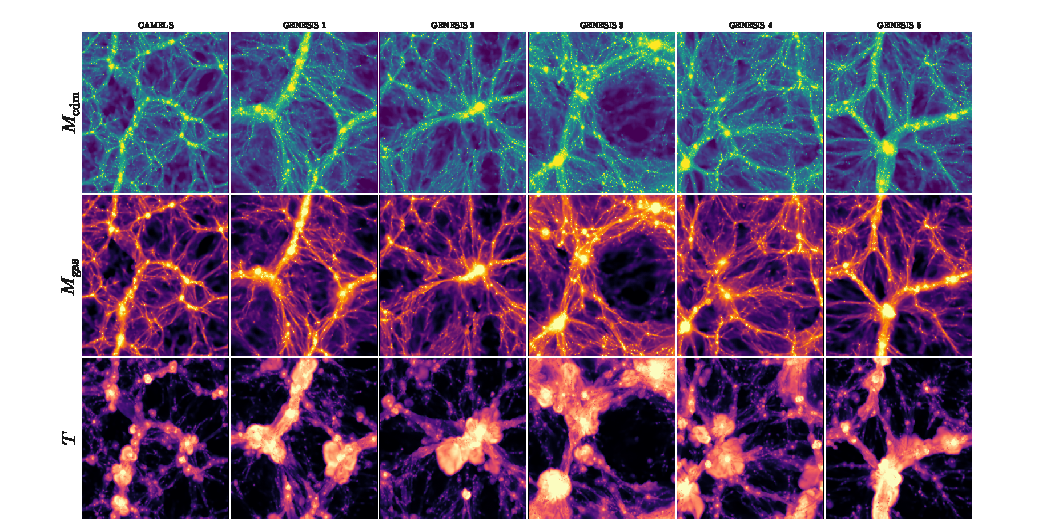
\includegraphics[width=\textwidth]{figs/lh/lh_tiles.pdf}
  \caption{
  Comparison between Camels LH map and Genesis generated map. The
  first column shows a CAMELS map triplet, while the remaining columns
  show independent \textsc{Genesis} samples generated at the same
  conditioning vector,
  $(\Om,\sig,A_{\rm SN1},A_{\rm SN2},A_{\rm AGN1},A_{\rm AGN2})
  =(0.3542,0.8706,1.3398,0.8839,1.0785,1.0063)$.
  Rows show $\Mcdm$, $\Mgas$, and $\Tgas$.
  }
  \label{fig:lh_tiles}
\end{figure*}

Training therefore minimizes
\begin{equation}
  \mathcal{L}_{\rm CFM} =
  \mathbb{E}_{t\sim\mathcal{U}(0,1),\,
  \mathbf{x}_0\sim p_0,\,
  \mathbf{x}_1\sim q(\mathbf{x}_1\mid\thetavec)}
  \left\|
    u_t^\phi(\mathbf{x}_t\mid\thetavec)
    - (\mathbf{x}_1-\mathbf{x}_0)
  \right\|^2 .
  \label{eq:cfm}
\end{equation}

\textbf{Sampling.}
After training, to generate a sample at a specified
conditioning vector $\thetavec$, we draw
$\mathbf{x}_0 \sim \mathcal{N}(\mathbf{0},\mathbf{I})$ and integrate
equation~(\ref{eq:flow_ode}) from $t=0$ to $t=1$ using the
Dormand--Prince (\texttt{dopri5}) adaptive Runge--Kutta solver with
relative and absolute tolerances of $10^{-5}$. The terminal state
$\mathbf{x}_{1}$ is interpreted as a sample from the learned
conditional data distribution. For the CV sampling runs used below,
generating 200 independent multifield map triplets at a fixed
conditioning vector takes roughly 20 minutes on a single NVIDIA A100
GPU, corresponding to about 6 seconds per triplet in the current
implementation.

\textbf{Classifier-free guidance.}
Classifier-free guidance \citep[CFG;][]{Ho2022} is commonly used in
conditional generation by training a model on both conditional and
unconditional inputs. In the flow-matching setting, the same idea can
be applied at the level of the learned velocity field: a guided
velocity is formed by extrapolating the conditional velocity away from
the unconditional one,
\begin{equation}
  \hat{u}_t
  =
  u_t^\phi(\mathbf{x}_t \mid \thetavec_\varnothing)
  + w\left[
    u_t^\phi(\mathbf{x}_t \mid \thetavec)
    - u_t^\phi(\mathbf{x}_t \mid \thetavec_\varnothing)
  \right],
  \label{eq:cfg}
\end{equation}
where $w$ is the guidance weight and $\thetavec_\varnothing$ denotes
the null token. Values $w>1$ strengthen the influence of the
conditioning vector by amplifying the difference between the
conditional and unconditional velocity predictions.
During training, we randomly replace the CAMELS conditioning vector
$\thetavec$ with $\thetavec_\varnothing$ with probability
$p_{\rm cfg}=0.1$, exposing the network to both conditional and
unconditional velocity prediction tasks. In this work we set $w=1$ at
inference, which recovers the standard conditional velocity
$\hat{u}_t = u_t^\phi(\mathbf{x}_t \mid \thetavec)$ without
extrapolation. Thus, the null-token branch is used primarily as a
training-time conditioning dropout mechanism rather than as an
inference-time guidance boost. Empirically, retaining this branch
improved both the validation loss and the statistical quality of
generated samples, suggesting that exposure to unconditional inputs
regularizes the learned velocity field.

\begin{figure*}
  \centering
  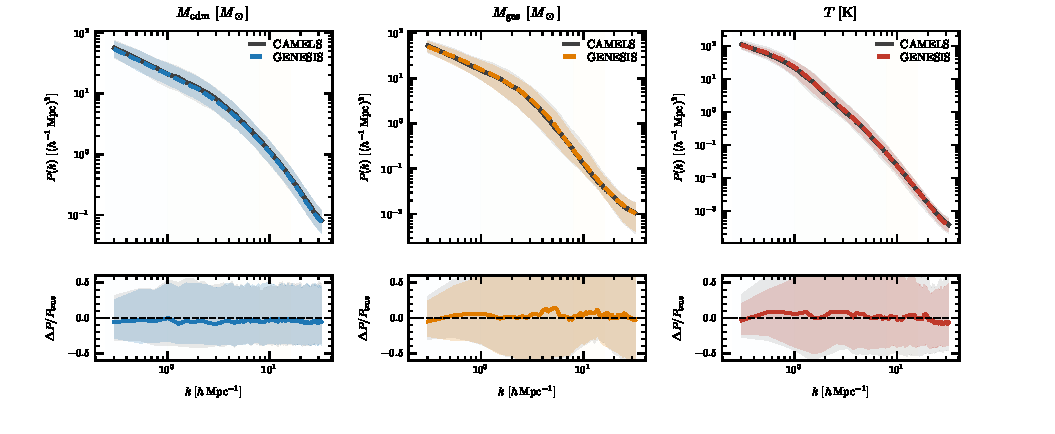
\includegraphics[width=\textwidth]{figs/lh/lh_autopk.pdf}
  \caption{
  Auto-power spectra and fractional residuals on the LH test set.
  Top panels show the LH-aggregated CAMELS and \textsc{Genesis} auto-power
  spectra for $\Mcdm$, $\Mgas$, and $\Tgas$ after aggregating over the
  100 held-out LH conditioning vectors. Bottom panels show
  $\epsilon_P(k)$, the fractional difference between the LH-aggregated
  mean spectra defined in equation~(\ref{eq:lh_auto_eps}).
  }
  \label{fig:lh_autopk}
\end{figure*}

\subsection{U-Net architecture}
\label{sec:architecture}
We parameterize the velocity field $u_t^\phi$ with a U-Net
architecture equipped with skip connections \citep{Ronneberger2015}.
The network takes as input the interpolated field
$\mathbf{x}_t \in \mathbb{R}^{3 \times 256 \times 256}$, the flow
time $t$, and the conditioning vector $\thetavec \in \mathbb{R}^6$.
The flow time $t$ is mapped to a sinusoidal embedding, and the
conditioning vector $\thetavec$ is mapped through a four-layer MLP,
each to 512 dimensions. These embeddings are concatenated and
projected through an MLP $(1024 \rightarrow 1024 \rightarrow 512)$ to
form a shared time--condition embedding $\mathbf{e}_{\rm joint}$.

We augment this backbone with three physically motivated design
choices. \textbf{Circular convolutions.}
The projected maps inherit periodic boundary conditions from the
CAMELS simulation volume \citep{Villaescusa2022}. We therefore use
circular padding in all convolutional layers, reducing boundary
artefacts that would be introduced by zero or reflective padding.
\textbf{Stage-wise conditioning.}
At each resolution level, we start from the shared time--condition
embedding $\mathbf{e}_{\rm joint}$ and augment it with a
stage-specific projection of the conditioning embedding,
\begin{equation}
  \boldsymbol{\ell}_i
  =
  \mathbf{e}_{\rm joint} + W_i(\mathbf{c}_{\rm emb}),
  \label{eq:stage_embedding}
\end{equation}
where $\mathbf{c}_{\rm emb}$ denotes the conditioning embedding and
$W_i$ is a learned linear adapter for stage $i$. The
resulting level embedding $\boldsymbol{\ell}_i$ is then used to
modulate the GroupNorm \citep{Wu2018} output at every residual block
via learned affine scale and shift parameters \citep[FiLM;][]{Perez2018}.
This allows each resolution level to interpret the conditioning
information differently: coarse stages govern large-scale morphology
and power-spectrum amplitude, while finer stages modulate small-scale
texture and the spatial extent of feedback-driven features.
\textbf{Scale-limited self-attention.}
Self-attention \citep{Vaswani2017} is applied at $64\times64$
resolution and below, including the bottleneck and corresponding
decoder stages. By computing pairwise similarities across all spatial
positions, it captures the long-range correlations and
inter-field dependencies that local convolutions cannot reach.
The final architecture has four encoder stages with channel widths
$[128, 256, 384, 512]$, two residual blocks per encoder stage,
strided circular convolutions for downsampling, a
residual--attention--residual bottleneck, and a symmetric decoder
with skip concatenations. The network maps three input channels to
three output velocity channels and contains approximately $93.0$
million trainable parameters.
% We also tested a Swin Transformer backbone \citep{Liu2021}; in our
% experiments it did not improve the validation metrics and was slower at
% inference, so we adopt the U-Net backbone for all results below.

\subsection{Training}
\label{sec:training}

We train \textsc{Genesis} in three stages. The initial training stage
uses AdamW \citep{Loshchilov2019} with learning rate
$\eta=2\times10^{-4}$, weight decay $10^{-2}$, and
$(\beta_1,\beta_2)=(0.9,0.999)$. The learning rate is warmed up for
5 epochs and then controlled by a ReduceLROnPlateau scheduler. This
stage is run for 89 epochs. We then perform two fine-tuning stages. The first fine-tuning stage
uses a smaller learning rate, $\eta=2\times10^{-5}$, no warm-up, and
a ReduceLROnPlateau scheduler with factor $0.65$ and patience 4. This
stage is run for 42 epochs. The final fine-tuning stage starts from
the first fine-tuned model and disables classifier-free conditioning
dropout by setting $p_{\rm cfg}=0$. This stage is run for 25 epochs
and provides the checkpoint used for all results reported in this
work. All stages use batches of $B=16$ multifield map triplets and D4 data
augmentation. Training is performed on a single NVIDIA A100 GPU.

%% =============================================================
%%  §4  LH EVALUATION
%% =============================================================
\section{LH evaluation}
\label{sec:eval}

This section evaluates \textsc{Genesis} on the held-out CAMELS/CMD
Latin-hypercube (LH) test set. The LH test set contains 100 held-out
simulations, each with 15 projected multifield map triplets; for each
conditioning vector we generate 30 \textsc{Genesis} samples.
Section~\ref{sec:eval_morphology} presents representative generated
map triplets, Section~\ref{sec:eval_autopower} compares the
auto-power spectra of the three target fields,
Section~\ref{sec:eval_onepoint} evaluates one-point field
distributions and mean amplitudes,
Section~\ref{sec:eval_cross_coherence} examines cross-power spectra
and inter-field coherence, and Section~\ref{sec:eval_response}
assesses the conditional parameter response and ensemble spread.

\subsection{Field morphology}
\label{sec:eval_morphology}

We begin with a visual comparison of \textsc{Genesis} maps from the
LH test set. Since \textsc{Genesis} is a stochastic generator, the
generated maps are not expected to reconstruct the same realization
as the CAMELS maps. Instead, this comparison checks whether samples
generated at the same conditioning vector exhibit similar field
morphology and cross-field structure.

Figure~\ref{fig:lh_tiles} shows that \textsc{Genesis} produces
visually plausible samples with filamentary dark-matter structure,
and gas distributions tracing the cosmic web. The generated maps
differ from the CAMELS map at the realization level, as expected for
a stochastic generator without initial-condition conditioning. The
dark-matter and gas-density channels show comparable large-scale
morphology, while the temperature channel exhibits softer small-scale
features in the generated samples, a qualitative impression that we
revisit quantitatively in Section~\ref{sec:eval_response}.

\subsection{Auto-power spectra}
\label{sec:eval_autopower}

We next compare the auto-power spectrum $P_a(k)$ of each target field
$a\in\{\Mcdm,\Mgas,\Tgas\}$. Here $P_a(k)$ is computed from the
two-dimensional overdensity field of each map and azimuthally averaged
in Fourier space. This statistic measures the scale-dependent
fluctuation amplitude of each field, providing a direct test of whether
the generated maps reproduce the clustering strength of dark matter,
gas, and temperature structures.

In this subsection, we aggregate over the 100 held-out LH conditioning
vectors. Thus, the comparison tests the marginal distribution of
power spectra across the LH test set. The parameter-dependent response is examined
separately in Section~\ref{sec:eval_response}. For each field, we
compute the fractional difference between the LH-aggregated
\textsc{Genesis} and CAMELS mean auto-power spectra,
\begin{equation}
  \epsilon_P(k)
  =
  \frac{
  \left|
  \left\langle P_a^{\rm gen}(k;\theta)\right\rangle_{\theta}
  -
  \left\langle P_a^{\rm true}(k;\theta)\right\rangle_{\theta}
  \right|
  }{
  \left\langle P_a^{\rm true}(k;\theta)\right\rangle_{\theta}
  },
  \label{eq:lh_auto_eps}
\end{equation}
where the average is taken over the held-out LH conditioning vectors.
We then average $\epsilon_P(k)$ within three reporting bands:
low-$k$ ($k<1$), mid-$k$ ($1\leq k<8$), and high-$k$
($8\leq k<k_{\rm art}$), with $k$ in units of
$h\,{\rm Mpc}^{-1}$ and $k_{\rm art}\simeq 16$ denoting the upper
edge used before the reference-only artefact regime.

Figure~\ref{fig:lh_autopk} shows that the generated auto-power spectra
closely follow the LH-aggregated CAMELS reference spectra for all
three fields. The
dark-matter channel provides the cleanest gravitational baseline, with
particularly small residuals at high $k$. The baryonic fields,
$\Mgas$ and $\Tgas$, are more sensitive to supernova and AGN feedback,
but their generated spectra remain close to the CAMELS reference over
the reported scale bands.

\begingroup
  \centering
  \refstepcounter{table}
  \label{tab:lh_metrics}
  \begin{tabular}{lcccccc}
    \hline\hline
    Channel & $\bar{\epsilon}_P^{\mathrm{low}}$ & $\bar{\epsilon}_P^{\mathrm{mid}}$ & $\bar{\epsilon}_P^{\mathrm{high}}$ & KS & JSD & $R^2$ \\
    \hline
    $M_{\mathrm{cdm}}$ & 3.9\% & 2.1\% & 0.5\% & 0.0336 & 0.00262 & 0.842 \\
    $M_{\mathrm{gas}}$ & 4.2\% & 5.3\% & 4.7\% & 0.0364 & 0.00293 & 0.882 \\
    $T$ & 2.7\% & 1.9\% & 3.6\% & 0.0464 & 0.00454 & 0.833 \\
    \hline
  \end{tabular}
  \par\smallskip
  \parbox{\columnwidth}{\small
    \textbf{Table~\thetable.} Quantitative evaluation on the LH test set
    ($N_{\mathrm{sim}}=100$, $n_{\mathrm{gen}}=30$ per sim).
    Auto-$P(k)$ errors $\bar{\epsilon}_P$ are band-averaged fractional
    differences between the LH-aggregated CAMELS and \textsc{Genesis}
    mean auto-power spectra, following equation~(\ref{eq:lh_auto_eps}).
    KS and JSD measure pixel-value distribution fidelity. $R^2$ is the
    overall conditional response quality.}
\endgroup


The band-averaged errors in Table~\ref{tab:lh_metrics} summarize the
fractional difference between the LH-aggregated CAMELS and
\textsc{Genesis} mean spectra. For $\Mcdm$, the residuals are $3.9$,
$2.1$, and $0.5$ per cent in the low-, mid-, and high-$k$ bands,
respectively. For $\Mgas$, the corresponding residuals are $4.2$,
$5.3$, and $4.7$ per cent, while for $\Tgas$ they are $2.7$, $1.9$,
and $3.6$ per cent. These values therefore measure agreement with the
marginal spectral distribution over the held-out LH set. The $R^2$
column in Table~\ref{tab:lh_metrics} instead summarizes the
conditional response in log-power space and is discussed in
Section~\ref{sec:eval_response}. Overall, the auto-power spectra
indicate that \textsc{Genesis} reproduces the marginal distribution of
scale-dependent fluctuation amplitudes across the held-out LH
parameter space.

\subsection{One-point field distributions and mean amplitudes}
\label{sec:eval_onepoint}

The auto-power spectra above are computed from overdensity fields and
therefore primarily test relative spatial fluctuations. We therefore
also examine one-point field statistics in physical field space. These
diagnostics test whether \textsc{Genesis} reproduces the absolute
amplitude range of each field, including dense matter and gas regions
as well as the high-temperature tail of shock- and feedback-heated
gas.

\begin{figure}
  \centering
  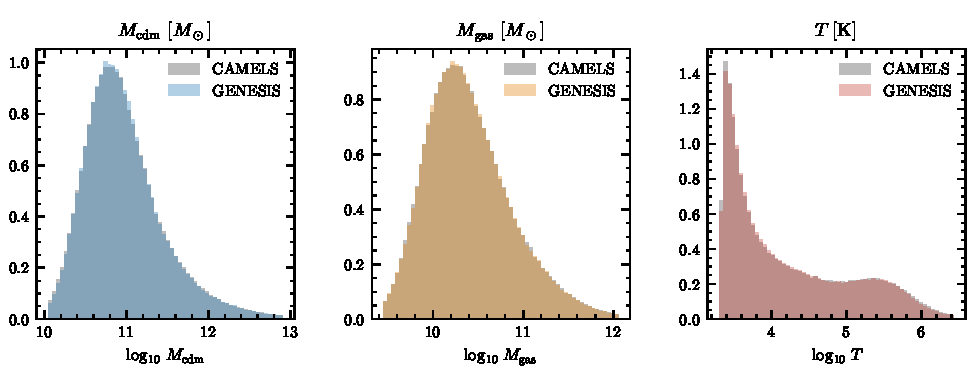
\includegraphics[width=\columnwidth]{figs/lh/lh_pixel_hist.pdf}
  \caption{
  One-point pixel distributions on the LH test set in $\log_{10}$ field
  space. Grey histograms show CAMELS and coloured histograms show
  \textsc{Genesis}.
  }
  \label{fig:lh_pixel_hist}
\end{figure}

Figure~\ref{fig:lh_pixel_hist} shows that the pixel
distributions of \textsc{Genesis} and CAMELS are very similar for all
three target fields. The $\Mcdm$ and $\Mgas$ distributions nearly
overlap, while $\Tgas$ is more challenging due to the combination of cold
diffuse gas with shock- and feedback-heated material. Nevertheless,
the \textsc{Genesis} temperature distribution reproduces the distribution of CAMELS, including its extended high-temperature tail and two modes.

We then compare the pixel distributions in $\log_{10}$ field space using
the Kolmogorov--Smirnov statistic $D_{\rm KS}$, the Jensen--Shannon
divergence (JSD), and the relative errors in the mean and standard
deviation,
\begin{equation}
  \varepsilon_\mu
  =
  \frac{|\mu_{\rm gen}-\mu_{\rm true}|}{|\mu_{\rm true}|},
  \qquad
  \varepsilon_\sigma
  =
  \frac{|\sigma_{\rm gen}-\sigma_{\rm true}|}{\sigma_{\rm true}}.
  \label{eq:pixel_errors}
\end{equation}

\begin{table*}
  \centering
  \small
  \setlength{\tabcolsep}{4pt}
  \renewcommand{\arraystretch}{1.08}
  \begin{tabular*}{\textwidth}{@{\extracolsep{\fill}}lccc@{}}
    \toprule
    Metric & $M_{\mathrm{cdm}}$ & $M_{\mathrm{gas}}$ & $T$ \\
    \midrule
    KS stat $D$ & $0.0292$ $[0.0135,\ 0.0574]$ (82\%) & $0.0328$ $[0.0149,\ 0.0568]$ (78\%) & $0.0408$ $[0.0214,\ 0.0734]$ (58\%) \\
    $\varepsilon_\mu$ & $0.0018$ $[0.0006,\ 0.0038]$ (100\%) & $0.0022$ $[0.0007,\ 0.0047]$ (100\%) & $0.0097$ $[0.0034,\ 0.0231]$ (100\%) \\
    $\varepsilon_\sigma$ & $0.0171$ $[0.0044,\ 0.0363]$ (100\%) & $0.0161$ $[0.0044,\ 0.0441]$ (99\%) & $0.0247$ $[0.0070,\ 0.0570]$ (98\%) \\
    JSD & $0.0020$ $[0.0014,\ 0.0039]$ & $0.0022$ $[0.0014,\ 0.0041]$ & $0.0038$ $[0.0022,\ 0.0063]$ \\
    \bottomrule
  \end{tabular*}
  \caption{LH test-set pixel-value distribution statistics
    ($N_{\mathrm{sim}}=100$, $n_{\mathrm{gen}}=30$ per sim). Each cell reports
    the median and 68\% interval [p$_{16}$, p$_{84}$] over the 100 simulations.
    Pass\% indicates the fraction of simulations below the acceptance threshold
    (KS\,$\leq\!0.05$; $\varepsilon_\mu\!\leq\!0.05$;
    $\varepsilon_\sigma\!\leq\!0.10$). JSD has no threshold and is reported for
    reference.}
  \label{tab:lh_pdf}
\end{table*}

Table~\ref{tab:lh_pdf} summarizes these one-point statistics across
the 100 LH test simulations. The median KS statistics are $0.0292$,
$0.0328$, and $0.0408$ for $\Mcdm$, $\Mgas$, and $\Tgas$,
respectively, while the corresponding JSD values are $0.0020$,
$0.0022$, and $0.0038$. The mean field amplitudes are also accurately
reproduced: the median relative mean errors are $0.0018$, $0.0022$,
and $0.0097$ for $\Mcdm$, $\Mgas$, and $\Tgas$. The relative errors
in the pixel standard deviation remain small as well, with median
values of $0.0171$, $0.0161$, and $0.0247$. Thus, \textsc{Genesis}
matches not only the spatial fluctuations measured by $P(k)$, but
also the absolute amplitude scale and width of the one-point field
distributions.

\begin{figure}
  \centering
  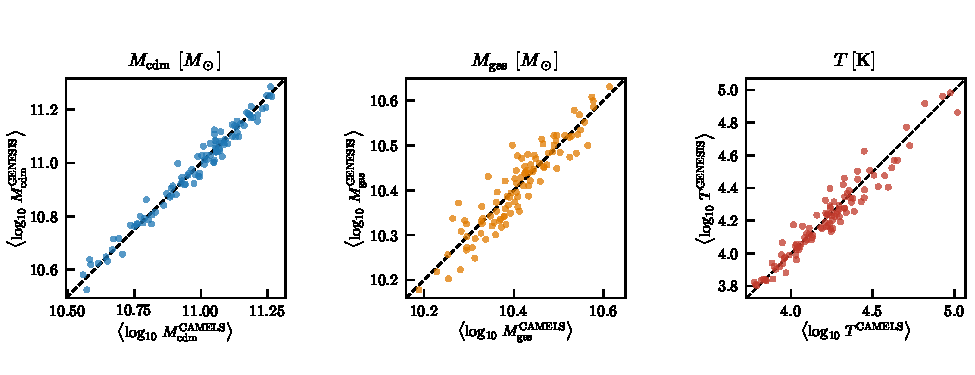
\includegraphics[width=\columnwidth]{figs/lh/lh_pixel_mean.pdf}
  \caption{Per-simulation mean field values on the LH test set. Each point
  corresponds to one held-out conditioning vector. The dashed line
  marks the one-to-one relation between CAMELS and \textsc{Genesis}.}
  \label{fig:lh_pixel_mean}
\end{figure}

Figure~\ref{fig:lh_pixel_mean} compares the mean field value for each
held-out conditioning vector. The points lie close to the one-to-one
relation for all three channels, showing that \textsc{Genesis} tracks
the parameter-dependent mean amplitude of the CAMELS maps. The
agreement is tightest for $\Mcdm$, while $\Mgas$ and $\Tgas$ show
larger scatter, consistent with their stronger sensitivity to
astrophysical feedback.

\subsection{Cross-power spectra and inter-field coherence}
\label{sec:eval_cross_coherence}

The preceding diagnostics test each field individually. We now ask
whether the three generated fields are mutually consistent. This is
essential for a multifield emulator: matching the auto-power spectra
and one-point distributions of $\Mcdm$, $\Mgas$, and $\Tgas$
separately does not guarantee that their spatial correlations are
correct.

We quantify the joint structure using the cross-power spectrum
\begin{equation}
  P_{ab}(k)
  =
  {\rm Re}
  \left[
  \left\langle
  \tilde{\delta}_a(\mathbf{k})
  \tilde{\delta}_b^*(\mathbf{k})
  \right\rangle_{|\mathbf{k}|=k}
  \right],
  \label{eq:cross_power_eval}
\end{equation}
and the inter-field coherence
\begin{equation}
  r_{ab}(k)
  =
  \frac{P_{ab}(k)}
  {\sqrt{P_{aa}(k)P_{bb}(k)}}.
  \label{eq:coherence_eval}
\end{equation}
The cross-power measures the scale-dependent amplitude of shared
structure between two fields, while the coherence removes the
individual field amplitudes and isolates their normalized spatial
correlation.

\begin{figure}
  \centering
  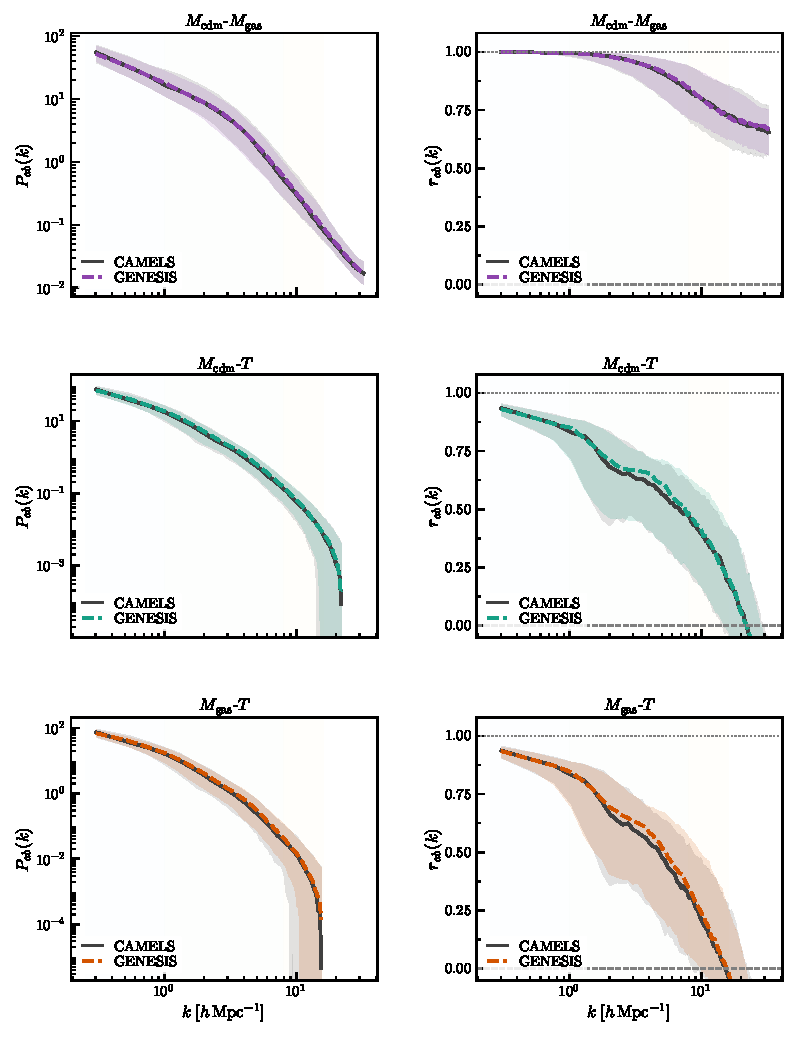
\includegraphics[width=\columnwidth]{figs/lh/lh_cross_coherence.pdf}
  \caption{
  Cross-power spectra and inter-field coherence on the LH test set.
  Left panels show $P_{ab}(k)$ and right panels show the coherence
  $r_{ab}(k)$ for the three field pairs
  $\Mcdm$--$\Mgas$, $\Mcdm$--$\Tgas$, and $\Mgas$--$\Tgas$.
  Black curves show CAMELS statistics and dashed coloured curves show
  \textsc{Genesis}; shaded regions indicate the 16--84 percentile
  ranges over the held-out LH set.
  }
  \label{fig:lh_cross_coherence}
\end{figure}

Figure~\ref{fig:lh_cross_coherence} shows that \textsc{Genesis}
reproduces the main cross-field correlations of the CAMELS maps. The
$\Mcdm$--$\Mgas$ pair is matched most closely, as expected from the
strong coupling between dark matter and gas density through the
underlying gravitational structure. The temperature-related pairs are
more challenging, because $\Tgas$ is affected not only by the density
field but also by shock heating and feedback processes. Nevertheless,
the generated cross-power spectra and coherence curves follow the
CAMELS trends across the reported scales.

This agreement indicates that \textsc{Genesis} does not merely
generate three plausible fields independently. Instead, the generated
map triplets preserve the correlated spatial structure among dark
matter density, gas density, and gas temperature. The largest visible
differences occur for temperature-related pairs, especially on smaller
scales where baryonic feedback introduces additional stochasticity.

\subsection{Conditional response and ensemble spread}
\label{sec:eval_response}

The diagnostics above show that \textsc{Genesis} reproduces the
marginal field statistics and the cross-field correlations of the LH
test set. We now examine whether the model also tracks how these
statistics vary across the six-dimensional CAMELS conditioning space.
For the auto-power spectrum, we quantify this response using
\begin{equation}
  R^2(k)
  =
  1 -
  \frac{
    {\rm MSE}_{\theta}
    \left[
      \log P_a^{\rm gen}(k;\theta)
      -
      \log P_a^{\rm true}(k;\theta)
    \right]
  }{
    {\rm Var}_{\theta}
    \left[
      \log P_a^{\rm true}(k;\theta)
    \right]
  },
  \label{eq:lh_r2}
\end{equation}
where the variance is taken over the 100 held-out LH simulations.
A value of $R^2=1$ indicates perfect tracking of the
parameter-dependent log-power response, while $R^2=0$ corresponds to
the performance of a parameter-independent mean prediction.

We also examine the normalized within-condition spread,
\begin{equation}
  S_{\rm cond}(k)
  =
  \left\langle
  \left[
  \frac{
    \log P_a^{\rm gen}(k;\theta)
    -
    \mu_a^{\rm true}(k;\theta)
  }{
    \sigma_a^{\rm true}(k;\theta)
  }
  \right]^2
  \right\rangle_{\theta},
  \label{eq:scond}
\end{equation}
where $\mu_a^{\rm true}$ and $\sigma_a^{\rm true}$ are computed from
the 15 CAMELS projections at the same conditioning vector. We use
$S_{\rm cond}$ as a diagnostic of within-condition ensemble spread
rather than as a formal calibration test. Since it is computed relative
to the CAMELS within-condition mean, it includes both generated
scatter and any residual mean offset. Values near unity indicate that
the normalized RMS deviation of the generated samples is comparable
to the CAMELS projection-level scatter.

\begin{figure}
  \centering
  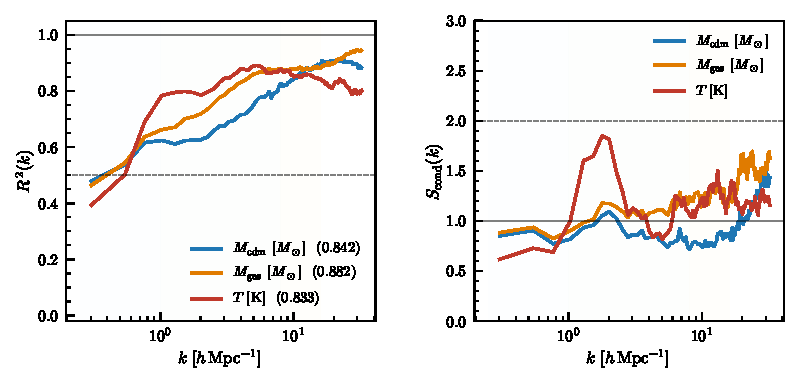
\includegraphics[width=\columnwidth]{figs/lh/lh_r2_scond.pdf}
  \caption{
  Conditional response and ensemble spread on the LH test set. Left:
  $R^2(k)$ of the generated log-power response across the held-out
  conditioning vectors. Right: $S_{\rm cond}(k)$, used here as a
  within-condition spread diagnostic.
  }
  \label{fig:lh_r2_scond}
\end{figure}

The left panel of Figure~\ref{fig:lh_r2_scond} shows that
\textsc{Genesis} tracks a substantial fraction of the
parameter-dependent variation in the log-power spectra. The overall
$R^2$ values are $0.842$, $0.882$, and $0.833$ for $\Mcdm$,
$\Mgas$, and $\Tgas$, respectively. To anchor these numbers, a
parameter-independent mean predictor that always returns the
LH-averaged log-power spectrum regardless of $\thetavec$ would have
$R^2=0$, while perfect tracking would give $R^2=1$. Thus, by this
metric, the conditioning in \textsc{Genesis} recovers approximately
83--88 per cent of the variance in log-power across the LH parameter
space.

Interestingly, the highest $R^2$ is obtained for $\Mgas$ rather than
for the gravitationally simpler $\Mcdm$ channel. This likely reflects
the stronger parameter response of the gas-density field across the
six-dimensional CAMELS design space. Supernova and AGN feedback
variations introduce substantial variation in
$\log P_{\rm gas}(k;\thetavec)$, increasing the denominator
${\rm Var}_{\theta}[\log P_a^{\rm true}(k;\theta)]$ in
equation~(\ref{eq:lh_r2}). By contrast, the dark-matter field is
sensitive primarily to $\Om$ and $\sig$ and only weakly to the
feedback parameters, so its conditional-variance denominator is
smaller. Comparable model errors can therefore lead to a slightly
lower $R^2$ for $\Mcdm$.

The right panel of Figure~\ref{fig:lh_r2_scond} shows that
$S_{\rm cond}$ remains broadly of order unity for much of the plotted
range, especially for $\Mcdm$. For the baryonic fields,
$S_{\rm cond}$ increases on feedback-sensitive scales, indicating
larger normalized RMS deviations from the CAMELS within-condition
mean. Values of $S_{\rm cond}\sim 2$ correspond to RMS deviations of
order $\sqrt{2}\simeq1.4$ times the CAMELS projection-level scatter,
although this quantity includes both generated scatter and any
residual mean offset. The largest departures are visible for $\Mgas$
and $\Tgas$, where feedback and thermal processes introduce
additional stochasticity. We therefore interpret this as mild
over-dispersion or residual bias in the most feedback-sensitive
regimes, rather than as a formal coverage statement.

Overall, the LH evaluation shows that \textsc{Genesis} reproduces the
main per-field and cross-field statistics of CAMELS across the
six-dimensional parameter space. The strongest agreement appears in
the auto-power spectra, one-point distributions, per-simulation field
means, and conditional log-power response. The largest remaining
discrepancies occur in feedback-sensitive baryonic statistics,
especially temperature-related correlations and small-scale ensemble
spread. Additional LH map tiles across a wider range of conditioning
vectors are shown in Appendix~\ref{app:lh_tiles}.

%%------------------------------------------------------------
\section{CV Evaluation}
\label{sec:cv_eval}

This section evaluates \textsc{Genesis} on the CAMELS/CMD CV set,
where all simulations share the same parameter vector $\thetavec$ but
differ in initial conditions. Section~\ref{sec:cv_tiles} presents
representative generated map triplets at the fiducial parameter point,
Section~\ref{sec:cv_auto_pk} compares the auto-power spectra,
Section~\ref{sec:cv_dcv} examines CV-normalized spectral displacement
and map-level spread, Section~\ref{sec:cv_pixel_pdf} compares
one-point field distributions, and Section~\ref{sec:cv_cross}
evaluates cross-power spectra and inter-field coherence. For the CV
comparisons, we generate 200 independent \textsc{Genesis} samples at
the fiducial conditioning vector; this takes roughly 20 minutes on a
single NVIDIA A100 GPU in the current implementation.

\subsection{Field morphology at fixed parameters}
\label{sec:cv_tiles}

As in the LH evaluation, we begin with a visual comparison of
\textsc{Genesis} maps from the CV set. Since the 27 CV simulations
themselves differ in initial conditions, the relevant question is
whether samples generated at the fiducial conditioning vector lie
within the morphological range spanned by independent CAMELS
realizations.

\begin{figure*}
  \centering
  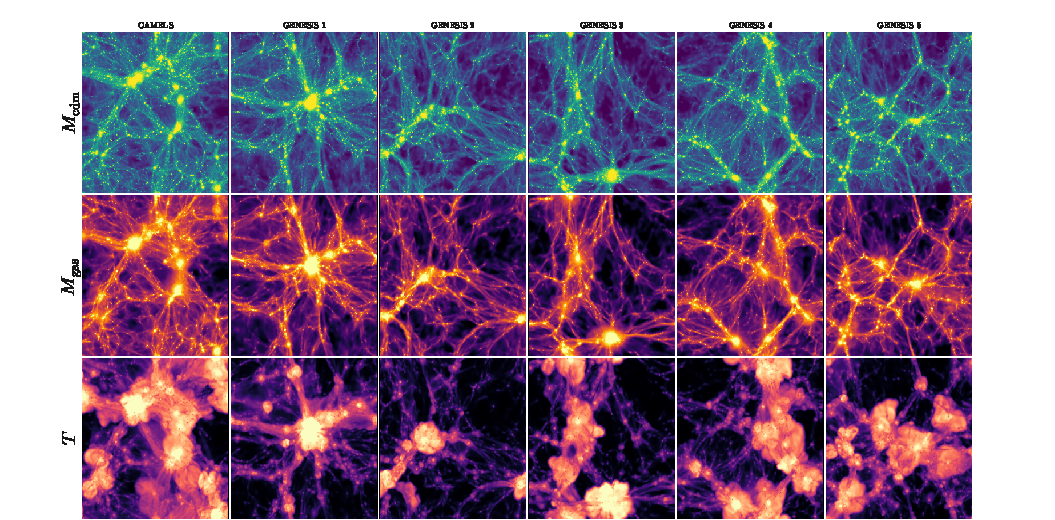
\includegraphics[width=\textwidth]{figs/cv/cv_tiles.pdf}
  \caption{
  Comparison between CAMELS CV map and Genesis generated map,conditoned on
  $(\Om,\sig,A_{\rm SN1},A_{\rm SN2},A_{\rm AGN1},A_{\rm AGN2})
  =(0.30,0.80,1,1,1,1)$. CAMELS realizations are compared with
  independent \textsc{Genesis} samples generated at the same
  conditioning vector. Rows show $\Mcdm$, $\Mgas$, and $\Tgas$.
  }
  \label{fig:cv_tiles}
\end{figure*}

Figure~\ref{fig:cv_tiles} shows that \textsc{Genesis} produces
visually plausible samples at the fiducial parameter point. The
dark-matter and gas-density channels show filamentary structure and
gas distributions that fall within the visual range of independent
CAMELS realizations. The temperature channel again shows softer
small-scale features in the generated samples, consistent with the
small-scale over-dispersion quantified in Section~\ref{sec:cv_dcv}.
The remaining subsections test this agreement more quantitatively
using summary statistics across the full CV set.

\subsection{Auto-power spectra}
\label{sec:cv_auto_pk}

We first compare the auto-power spectra of the generated maps with
those of the CAMELS CV maps. Since the CV set is evaluated at fixed
parameters, this comparison tests whether \textsc{Genesis} produces
samples with similar spectral statistics to independent CAMELS
realizations at the fiducial parameter point.

\begin{figure*}
  \centering
  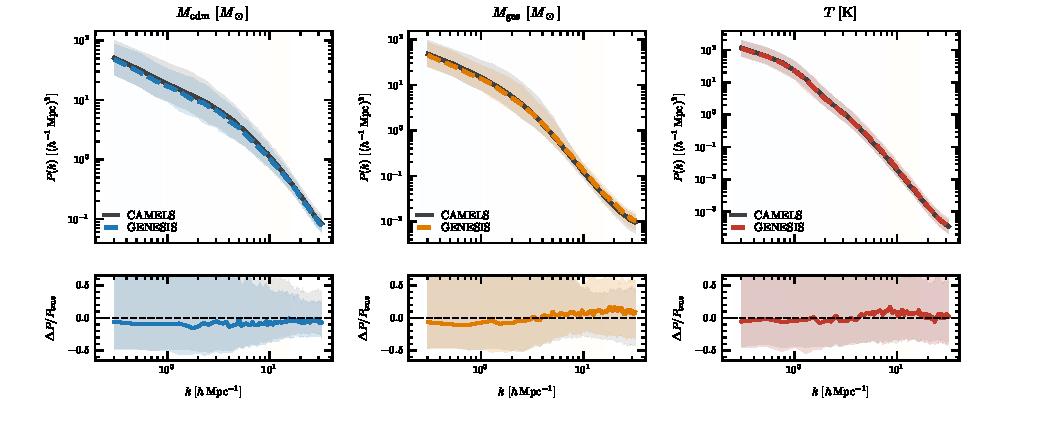
\includegraphics[width=\textwidth]{figs/cv/cv_auto_pk.pdf}
  \caption{
  Auto-power spectra on the CV set. Top panels show CAMELS and
  \textsc{Genesis} auto-power spectra for $\Mcdm$, $\Mgas$, and
  $\Tgas$; shaded regions indicate the 16--84 percentile ranges.
  Bottom panels show fractional residuals relative to the CAMELS
  median.
  }
  \label{fig:cv_auto_pk}
\end{figure*}

Figure~\ref{fig:cv_auto_pk} shows that the generated spectra follow
the CAMELS medians for all three fields. The residuals are generally
small compared with the map-level scatter, although mild
scale-dependent differences remain. For $\Mcdm$, the residual is
slightly below zero over most of the plotted range, indicating a small
low-power bias in the generated dark-matter spectra. The baryonic
fields show additional scale-dependent departures, as expected from
their stronger sensitivity to feedback and thermal processes.
Overall, the generated samples reproduce the main two-point
clustering amplitudes at the fiducial CV parameter point, with these
residual trends indicating mild field-dependent biases rather than
large failures.

\subsection{CV-normalized displacement and map-level spread}
\label{sec:cv_dcv}

We further summarize the spectral comparison using a CV-normalized
displacement,
\begin{equation}
  d_{{\rm CV},a}(k)
  =
  \frac{
    \langle P_a^{\rm gen}(k)\rangle_{\rm gen}
    -
    \langle \overline{P}_{a,j}^{\rm CV}(k)\rangle_j
  }{
    {\rm std}_j[\overline{P}_{a,j}^{\rm CV}(k)]
  },
  \label{eq:dcv}
\end{equation}
where $\overline{P}_{a,j}^{\rm CV}(k)$ denotes the mean auto-power
spectrum of the 15 projected maps from CV simulation $j$. This
quantity measures the displacement of the generated mean spectrum in
units of the simulation-to-simulation scatter among the CV runs.

We also consider a map-level spread ratio,
\begin{equation}
  R_{\sigma,a}(k)
  =
  \frac{
    {\rm Var}_{\rm gen}[\log P_a(k)]
  }{
    {\rm Var}_{\rm CV,map}[\log P_a(k)]
  }.
  \label{eq:rsigma_cv}
\end{equation}
We use \(R_\sigma\) only as a diagnostic of relative spread. The
CAMELS CV maps include both realization-to-realization variation and
projection-level scatter, while the generated maps are independent
samples from the learned conditional model.

\begin{figure}
  \centering
  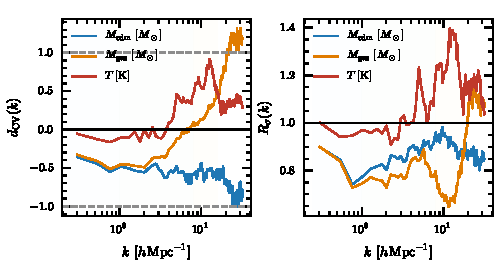
\includegraphics[width=\columnwidth]{figs/cv/cv_dcv_rsigma.pdf}
  \caption{
  CV-normalized spectral displacement and map-level spread. Left:
  $d_{\rm CV}(k)$ for the generated mean auto-power spectrum. Right:
  $R_\sigma(k)$, the ratio of generated to CAMELS map-level
  log-power variance.
  }
  \label{fig:cv_dcv_rsigma}
\end{figure}

Figure~\ref{fig:cv_dcv_rsigma} shows that $d_{\rm CV}$ provides a
directional measure of bias at the fiducial parameter point. The
dark-matter channel exhibits a coherent $d_{\rm CV}\simeq -0.5$
across most scales, indicating that the \textsc{Genesis} mean
spectrum lies roughly half of the CV simulation-to-simulation scatter
below the CAMELS mean. This is a systematic but mild underprediction.
The gas-density channel reaches $d_{\rm CV}\simeq -1$ on some scales,
suggesting that the bias can approach the level of the intrinsic CV
scatter. The temperature channel remains closer to unbiased, with
$d_{\rm CV}$ varying around zero and becoming mildly positive toward
high $k$.

The map-level spread ratio $R_\sigma$ gives a complementary view of
the generated ensemble. For $\Mcdm$, $R_\sigma\simeq 0.8$, indicating
that the generated samples are slightly less dispersed than the
CAMELS map-to-map variation. For $\Mgas$, $R_\sigma$ remains close to
unity, showing well-matched map-level spread. For $\Tgas$, $R_\sigma$
increases to approximately $1.4$ on small scales, indicating broader
generated temperature fluctuations where feedback and thermal
processes dominate. This small-scale over-dispersion is consistent
with the elevated $S_{\rm cond}$ values seen for the LH set in
Section~\ref{sec:eval_response}. Together, the two CV diagnostics
suggest a coherent picture: \textsc{Genesis} slightly underestimates
the dark-matter clustering amplitude at the fiducial point, matches
the gas-density spread well, and over-disperses temperature on
feedback-sensitive small scales.

\subsection{One-point field distributions}
\label{sec:cv_pixel_pdf}

We next compare one-point pixel distributions in $\log_{10}$ field
space. This complements the power-spectrum comparison by testing the
absolute range of field values rather than only relative fluctuations
in overdensity.

\begin{figure}
  \centering
  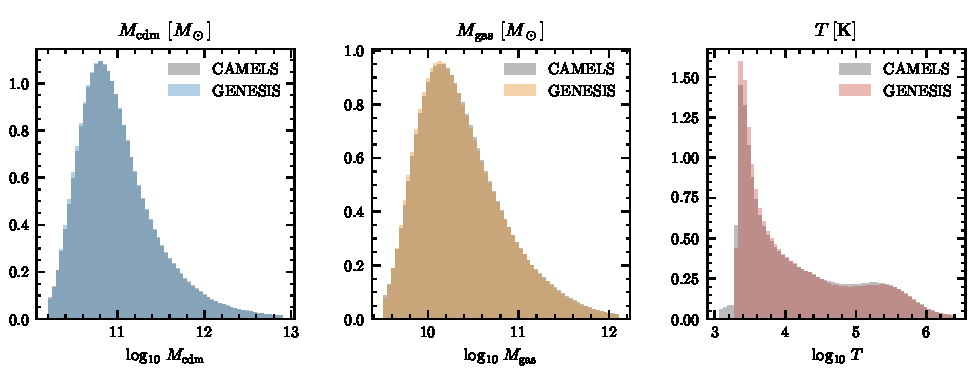
\includegraphics[width=\columnwidth]{figs/cv/cv_pixel_pdf.pdf}
  \caption{
  One-point pixel distributions on the CV set in $\log_{10}$ field
  space. Grey histograms show CAMELS and coloured histograms show
  \textsc{Genesis}.
  }
  \label{fig:cv_pixel_pdf}
\end{figure}

Figure~\ref{fig:cv_pixel_pdf} shows similar CAMELS and
\textsc{Genesis} pixel distributions for all three fields. The
agreement is particularly close for the two density fields. The
temperature distribution is broader and more structured, but the
generated samples still follow its main shape. This suggests that the
model captures the typical field amplitudes at the fiducial parameter
point, while leaving some differences in the more feedback-sensitive
temperature field.

\subsection{Cross-power spectra and inter-field coherence}
\label{sec:cv_cross}

Finally, we examine the joint structure of the three generated fields.
We compare the cross-power spectra \(P_{ab}(k)\) and coherence
\(r_{ab}(k)\) for the field pairs
$\Mcdm$--$\Mgas$, $\Mcdm$--$\Tgas$, and $\Mgas$--$\Tgas$.

\begin{figure}
  \centering
  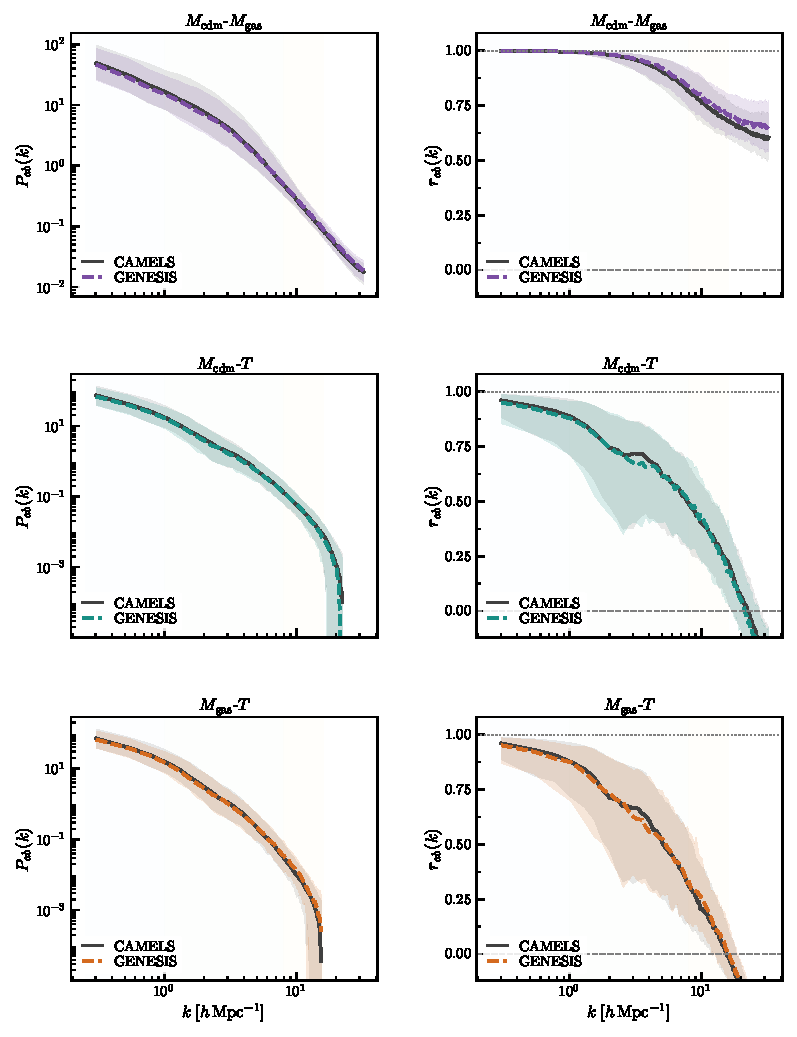
\includegraphics[width=\columnwidth]{figs/cv/cv_cross_coherence.pdf}
  \caption{
  Cross-power spectra and inter-field coherence on the CV set. Left
  panels show $P_{ab}(k)$ and right panels show the coherence
  $r_{ab}(k)$ for the three field pairs. Black curves show CAMELS and
  dashed coloured curves show \textsc{Genesis}; shaded regions
  indicate 16--84 percentile ranges.
  }
  \label{fig:cv_cross_coherence}
\end{figure}

Figure~\ref{fig:cv_cross_coherence} shows that the generated samples
broadly follow the CAMELS cross-field statistics. The
$\Mcdm$--$\Mgas$ pair shows the closest agreement, while the
temperature-related pairs show larger differences, particularly on
smaller scales. This is consistent with the greater sensitivity of
temperature to shock heating and feedback processes. Overall, the
comparison indicates that \textsc{Genesis} preserves the main
multifield correlations at the fiducial parameter point, with the
largest residuals appearing in the baryonic and temperature-related
statistics.

Taken together, the CV diagnostics show that \textsc{Genesis}
produces samples with broadly similar auto-power spectra, one-point
distributions, and cross-field correlations to CAMELS at the fiducial
parameter vector. The comparison also identifies remaining differences
in map-level spread and in temperature-related baryonic statistics.
The 200-sample CV ensemble is generated in roughly 20 minutes on a
single NVIDIA A100 GPU, indicating that forward sampling is practical
for moderate ensemble sizes even though likelihood evaluation remains
substantially more expensive.

%% =============================================================
%%  §6  LIKELIHOOD-BASED INFERENCE DEMONSTRATION
%% =============================================================
\section{Likelihood-based parameter inference}
\label{sec:likelihood_inference}

This section demonstrates likelihood-based parameter inference with
\textsc{Genesis} by fixing one observed CAMELS multifield map,
denoted $\mathbf{x}_1$, and scanning the cosmological parameters
$\Om$ and $\sig$. Section~\ref{sec:likelihood_change} describes likelihood
evaluation through the change-of-variables formula for continuous
normalizing flows, Section~\ref{sec:likelihood_hutchinson} describes
the Hutchinson trace estimator and the scan setup, and
Section~\ref{sec:likelihood_results} presents a two-dimensional
profile likelihood scan in the $\Om$--$\sig$ plane.

\subsection{Flow likelihood from change of variables}
\label{sec:likelihood_change}

\textsc{Genesis} is trained as a continuous normalizing flow so,
in principle, it can provide an explicit likelihood for a map at a
specified conditioning vector $\thetavec$. In the likelihood scan, the
observed map $\mathbf{x}_1$ is fixed and only the candidate
conditioning vector is changed.
The learned probability-flow ODE is
\begin{equation}
  \frac{\mathrm{d}\mathbf{x}_t}{\mathrm{d}t}
  =
  u_t^\phi(\mathbf{x}_t\mid\thetavec),
  \qquad t\in[0,1],
  \label{eq:likelihood_pfode}
\end{equation}
with $\mathbf{x}_0\sim p_0=\mathcal{N}(\mathbf{0},\mathbf{I})$ and
$\mathbf{x}_1$ in the data distribution. Along this flow, the
instantaneous change of log-density is
\begin{equation}
  \frac{\mathrm{d}}{\mathrm{d}t}
  \log p_t(\mathbf{x}_t\mid\thetavec)
  =
  -
  \nabla_{\mathbf{x}}\!\cdot
  u_t^\phi(\mathbf{x}_t\mid\thetavec).
  \label{eq:instantaneous_change}
\end{equation}
Equivalently, for likelihood evaluation we integrate the learned flow
in the reverse direction, from the fixed data point $\mathbf{x}_1$ to
the corresponding latent point $\mathbf{z}_1$ in the noise space. The
conditional log likelihood is then evaluated as
\begin{equation}
  \log p_\phi(\mathbf{x}_1\mid\thetavec)
  =
  \log p_0(\mathbf{z}_1)
  +
  \int_0^1
  \nabla_{\mathbf{x}_t}\!\cdot
  u_t^\phi(\mathbf{x}_t\mid\thetavec)
  \,\mathrm{d}t .
  \label{eq:cnf_likelihood}
\end{equation}
We report relative likelihoods,
\begin{equation}
  \Delta\log p(\thetavec)
  =
  \log p_\phi(\mathbf{x}_1\mid\thetavec)
  -
  \max_{\thetavec'}
  \log p_\phi(\mathbf{x}_1\mid\thetavec'),
  \label{eq:dlogp_scan}
\end{equation}
where the maximum is taken over the evaluated scan grid. Thus the
best grid point has $\Delta\log p=0$, and all other grid points have
negative values.

\subsection{Hutchinson trace estimation and scan setup}
\label{sec:likelihood_hutchinson}
The divergence term
$\nabla_{\mathbf{x}_t}\!\cdot
u_t^\phi(\mathbf{x}_t\mid\thetavec)$ in
equation~\eqref{eq:cnf_likelihood}
is the trace of the Jacobian of the velocity field,
\begin{equation}
  \nabla_{\mathbf{x}_t}\!\cdot
  u_t^\phi(\mathbf{x}_t\mid\thetavec)
  =
  {\rm Tr}\!\left[
    \frac{\partial u_t^\phi}{\partial \mathbf{x}}
  \right].
  \label{eq:trace_exact}
\end{equation}
Because the map dimensionality is large, computing the exact trace at
each ODE step is intractable. We therefore estimate this trace with
the Hutchinson estimator,
\begin{equation}
  {\rm Tr}\!\left[
    \frac{\partial u_t^\phi}{\partial \mathbf{x}}
  \right]
  =
  \mathbb{E}_{\boldsymbol{\epsilon}}
  \left[
    \boldsymbol{\epsilon}^{\mathsf T}
    \frac{\partial u_t^\phi}{\partial \mathbf{x}}
    \boldsymbol{\epsilon}
  \right],
  \qquad
  \mathbb{E}
  [\boldsymbol{\epsilon}\boldsymbol{\epsilon}^{\mathsf T}]
  =
  \mathbf{I}.
  \label{eq:hutchinson}
\end{equation}
In practice, we use Rademacher probe vectors and average over three
Hutchinson seeds at each grid point. The plotted likelihood surface
uses the seed-averaged value
\begin{equation}
  \overline{\log p}_{ij}
  =
  \frac{1}{3}
  \sum_{s=0}^{2}
  \log p_{\phi,s}
  (\mathbf{x}_1\mid\thetavec_{ij}),
  \label{eq:hutchinson_mean}
\end{equation}
and the scatter across the three seeds is used as a diagnostic of
stochastic trace-estimator noise.

We scan the two cosmological parameters $\Om$ and $\sig$, while
fixing the four astrophysical parameters to their true values. The
CAMELS map used in this scan has true conditioning vector
\begin{equation}
  \thetavec_{\rm true}
  =
  (0.3054,\,0.8090,\,3.7373,\,3.8106,\,1.3822,\,0.6639).
  \label{eq:scan_true_params}
\end{equation}
This parameter vector is close to the Planck 2018 cosmology. The
candidate grid is
\begin{equation}
\begin{aligned}
  \Om &\in
  \{0.1985,0.2199,0.2413,0.2626,0.2840,0.3054,
  \\
  &\qquad
    0.3268,0.3482,0.3695,0.3909,0.4123\},
  \\
  \sig &\in
  \{0.6000,0.6400,0.6800,0.7200,0.7600,0.8090,
  \\
  &\qquad
    0.8400,0.8800,0.9200,0.9600,1.0000\}.
\end{aligned}
  \label{eq:scan_grid}
\end{equation}
The full candidate grid contains $11\times11=121$ points. To avoid
evaluating points far from the region of interest, we restrict the
calculation to the ellipse
\begin{equation}
  \left(
  \frac{\Om-\Omega_{{\rm m},{\rm true}}}{0.04}
  \right)^2
  +
  \left(
  \frac{\sig-\sigma_{8,{\rm true}}}{0.07}
  \right)^2
  \leq 3^2 .
  \label{eq:scan_ellipse}
\end{equation}
This skips 28 points outside the ellipse and leaves 93 evaluated
grid points. Each likelihood is computed with the Dormand--Prince
solver using 100 function evaluations.

\subsection{Two-dimensional profile likelihood scan}
\label{sec:likelihood_results}
\begin{figure}
  \centering
  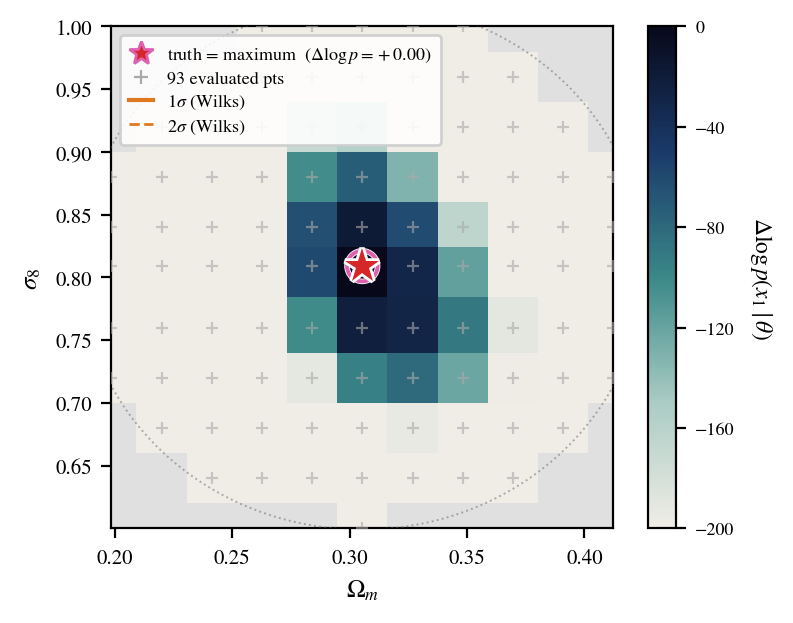
\includegraphics[width=\columnwidth]{figs/likelihood/scan2d_Omega_m_sigma_8_real_fig12_final.png}
  \caption{
  Two-dimensional likelihood scan in the $\Om$--$\sig$ plane for a
  fixed CAMELS map $\mathbf{x}_1$. The colour scale shows
  $\Delta\log p(\mathbf{x}_1\mid\thetavec)$ relative to the maximum
  evaluated grid value. The true CAMELS parameter and the
  maximum-likelihood grid point coincide at
  $(\Om,\sig)=(0.3054,0.8090)$. Grey regions indicate grid points
  outside the evaluated scan ellipse, and markers show evaluated grid
  points. Contours show the Wilks-theorem 1 and 2$\sigma$ levels for
  two parameters, corresponding to
  $\Delta\log p=-1.15$ and $-3.09$.
  }
  \label{fig:likelihood_scan_2d}
\end{figure}

Figure~\ref{fig:likelihood_scan_2d} shows that the seed-averaged
relative likelihood peaks at the true CAMELS parameter point,
$(\Om,\sig)=(0.3054,0.8090)$, which is included explicitly in the
scan grid. The colour scale shows the relative log likelihood, not an
absolute likelihood; values close to zero therefore correspond to
conditioning vectors that best explain the fixed map $\mathbf{x}_1$
within the evaluated grid. The surface is broad and the grey region
marks grid points skipped by the ellipse cut, so this result should
be interpreted as a proof-of-concept likelihood scan rather than a
precise cosmological constraint.

\begin{figure*}
  \centering
  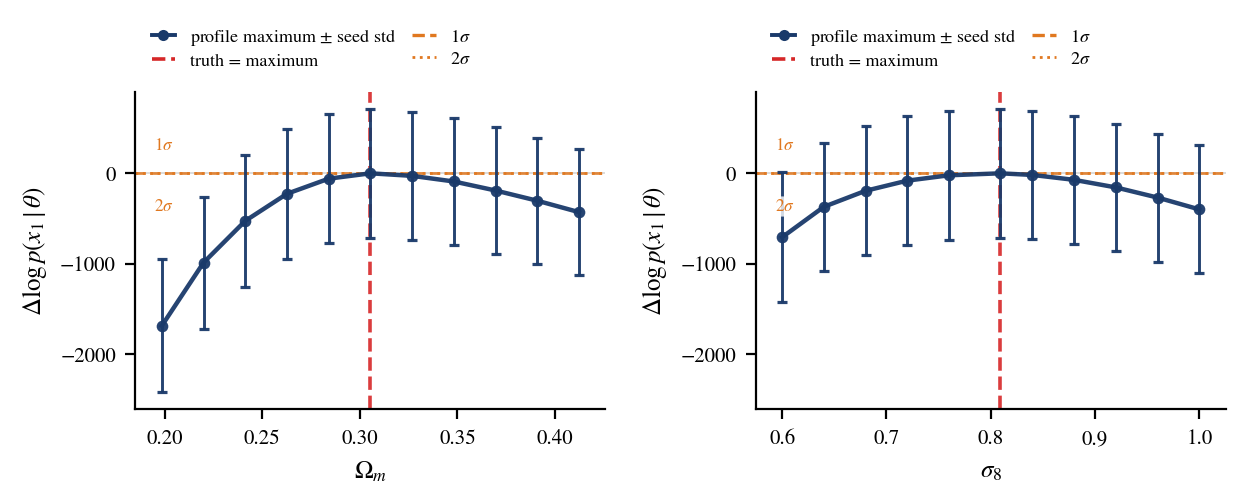
\includegraphics[width=\textwidth]{figs/likelihood/scan2d_Omega_m_sigma_8_real_fig13_final.png}
  \caption{
  One-dimensional profile projections of the likelihood scan. Left:
  profile in $\Om$, obtained by maximizing over $\sig$ at each
  $\Om$. Right: profile in $\sig$, obtained by maximizing over
  $\Om$ at each $\sig$. Error bars show the scatter across Hutchinson
  seeds. The vertical dashed line marks the CAMELS parameter value.
  Horizontal lines show the 1D Wilks-theorem 1 and 2$\sigma$ levels,
  $\Delta\log p=-0.5$ and $-2.0$.
  }
  \label{fig:likelihood_scan_profiles}
\end{figure*}

The profile projections in
Figure~\ref{fig:likelihood_scan_profiles} show the same qualitative
behaviour. For each value of one parameter, the profile keeps the
largest relative likelihood over the other parameter,
\begin{equation}
\begin{aligned}
  \Delta\log p_{\rm prof}(\Om)
  =
  \max_{\sig}
  \Delta\log p(\Om,\sig),
  \\
  \Delta\log p_{\rm prof}(\sig)
  =
  \max_{\Om}
  \Delta\log p(\Om,\sig).
\end{aligned}
  \label{eq:profile_likelihood}
\end{equation}
Both profiles peak at the true CAMELS value and remain broad, with
visible uncertainty from the stochastic trace estimator. This result
shows that the learned flow likelihood contains useful parameter
information for a low-dimensional scan on CAMELS data. A full
inference analysis would require sampling or scanning over the
remaining astrophysical parameters, more likelihood evaluations, and
calibration over multiple maps.

%% =============================================================
%%  §7  DISCUSSION
%% =============================================================
\section{Discussion and Further Work}
\label{sec:discussion}

The evaluations above show that \textsc{Genesis} can generate
multifield CAMELS maps whose summary statistics are broadly similar
to those of the target simulations. Across the LH test set, the model
matches the marginal auto-power spectra, one-point field
distributions, per-simulation mean amplitudes, and inter-field
correlations at the level of the diagnostics considered in this work.
The CV comparison gives a complementary fixed-parameter check,
showing that generated samples at the fiducial parameter point have
similar auto-power spectra, pixel distributions, and cross-field
statistics to independent CAMELS realizations.

At the same time, the residuals are not completely uniform across
fields or scales. In the CV auto-power spectra, the dark-matter field
shows a small but coherent tendency toward lower power relative to
the CAMELS median over part of the measured range, although the
band-averaged residuals remain at small levels. This suggests
that the model slightly underestimates some aspects of the dark-matter
fluctuation amplitude, rather than failing catastrophically in any
particular scale band. 

The cross-field diagnostics are particularly important for interpreting
the model as a multifield emulator. A model could reproduce the
auto-power spectra of $\Mcdm$, $\Mgas$, and $\Tgas$ separately while
still generating mutually inconsistent fields. The cross-power and
coherence results indicate that \textsc{Genesis} preserves the main
spatial coupling among the three fields. The agreement is strongest
for the $\Mcdm$--$\Mgas$ pair, while temperature-related pairs show
larger residuals, especially toward smaller scales. This behaviour is
consistent with the temperature field being more sensitive to local
heating and feedback processes than to density alone.

The likelihood scan demonstrates a separate aspect of the model:
because \textsc{Genesis} is formulated as a continuous normalizing
flow, the same trained model can be used to assign likelihoods to
input maps under candidate conditioning vectors. In the
two-dimensional $\Om$--$\sig$ scan, one CAMELS map $\mathbf{x}_1$ is
held fixed while the conditioning vector is varied over a restricted
grid that includes the true parameter point. The four astrophysical
feedback parameters are fixed to their true values, and the relative
likelihood is computed for the evaluated grid points inside a
$3\sigma$ ellipse around the CAMELS parameter value. The
maximum-likelihood grid point coincides with the truth,
$(\Om,\sig)=(0.3054,0.8090)$, and the Wilks-theorem 1$\sigma$
contour encloses several adjacent grid points. We therefore interpret
this result as a proof of concept that the likelihood surface is
centred on the truth at the resolution of the scan, rather than that
the truth is uniquely resolved within stochastic noise.

There are several limitations to this likelihood-based inference
demonstration. First, the scan varies only two cosmological parameters
and keeps the four astrophysical feedback parameters fixed. It is
therefore a low-dimensional profile likelihood slice, not a full
posterior analysis over the six-dimensional CAMELS parameter space. In
addition, only 93 of the 121 candidate grid points are evaluated after
applying the ellipse cut. The scan is therefore an encouraging
consistency check on the local likelihood surface, but not a
standalone validation of calibrated inference.

Second, likelihood evaluation is computationally expensive. In the
scan presented here, each conditioning vector requires an ODE solve
with stochastic divergence estimation, taking roughly two minutes on
an NVIDIA A100 GPU in the current implementation. The Hutchinson trace
estimator is unbiased and, when the random probe vectors are fixed,
gives a consistent relative trend across the scan, but it still
introduces non-negligible stochastic noise. Reducing this noise
requires averaging over more Hutchinson seeds, which directly
increases the runtime of each likelihood evaluation. Variance-reduction
strategies, improved ODE solvers, or learned approximations to the
likelihood surface may therefore be required for practical inference
applications.

A broader statistical limitation is that the current evaluation does
not yet provide a fully calibrated inference procedure. The LH and CV
diagnostics test whether generated fields reproduce selected summary
statistics, and the likelihood scan checks whether the CNF likelihood
peaks near the correct region for one CAMELS map. These tests are
useful, but they do not by themselves establish calibrated parameter
coverage, unbiased posterior means, or reliable credible intervals.
Such claims would require repeated inference experiments over many
maps, posterior calibration tests, and marginalization over all relevant
cosmological and astrophysical parameters.

The present work is also limited to two-dimensional projected maps
from a single simulation suite. Projection removes line-of-sight
information, and the $25\,h^{-1}{\rm Mpc}$ CAMELS volume limits the
available large-scale modes. Extending the approach to larger volumes
or three-dimensional fields would allow a more direct connection to
survey-scale clustering statistics, but would also require more memory
efficient architectures and more expensive validation. In addition,
\textsc{Genesis} is trained only on the IllustrisTNG branch of CAMELS.
Generalization to other hydrodynamic models, such as SIMBA or EAGLE,
would require retraining, transfer learning, or explicit multi-suite
training to separate cosmological dependence from baryonic model
dependence.

These limitations suggest several natural next steps. The CAMELS 1P
set can be used to test whether the generated fields reproduce
one-parameter response curves for each of the six conditioning
parameters. The EX set can test robustness near or outside the edges
of the LH training range. For likelihood-based inference, future work
should evaluate many CAMELS maps, scan or sample the full
six-dimensional parameter space, quantify estimator variance, and
check frequentist coverage or simulation-based calibration. These
steps are necessary before the likelihood can be used as a reliable
cosmological inference tool.

%% =============================================================
%%  §7  CONCLUSION
%% =============================================================
\section{Conclusions}
\label{sec:conclusions}

We have presented \textsc{Genesis}, a conditional generative emulator
for multifield cosmological maps based on optimal-transport flow
matching. The model jointly generates projected dark matter density,
gas density, and gas temperature fields, conditioned on the full
six-dimensional CAMELS parameter vector. We evaluated the model on
both the parameter-varying LH test set and the fixed-parameter CV set
using morphology, auto-power spectra, one-point statistics,
cross-field coherence, conditional response, and ensemble-spread
diagnostics.

Across these tests, \textsc{Genesis} reproduces the main CAMELS
statistics at a useful level. The generated maps match the marginal
auto-power spectra, one-point distributions, field means, and
cross-field structure reasonably well, and the conditional log-power
response tracks much of the variation across the LH parameter space.
The remaining discrepancies are concentrated in feedback-sensitive
baryonic quantities: temperature-related correlations and small-scale
temperature spread are less well matched, and the CV diagnostics show
a mild underprediction of dark-matter clustering amplitude at the
fiducial point. Thus, the model captures the dominant multifield
structure while still leaving clear targets for improved small-scale
baryonic modelling. In the current implementation, generating 200
independent multifield samples at a fixed conditioning vector takes
roughly 20 minutes on a single NVIDIA A100 GPU, showing that moderate
conditional ensembles are feasible.

We also demonstrated likelihood-based inference using the continuous
normalizing-flow change-of-variables formula. In a two-dimensional
$\Om$--$\sig$ scan with the astrophysical parameters fixed, the
likelihood maximum coincides with the true CAMELS parameter value for
the fixed observed map. This is not yet a calibrated cosmological
inference pipeline, but it shows that the learned flow likelihood
contains useful parameter information. Overall, these results indicate
that flow matching can be a promising tool for both conditional
cosmological field generation and field-level likelihood-based
inference.

%% =============================================================
%%  ACKNOWLEDGEMENTS
%% =============================================================
\section*{Acknowledgements}

M.P. acknowledges no external funding for this work.
Model training and evaluation were performed on the SKKU cluster using
personally funded computing resources.
This work made use of
\textsc{NumPy} \citep{Harris2020},
\textsc{SciPy} \citep{Virtanen2020},
\textsc{PyTorch} \citep{Paszke2019},
\textsc{Pylians3} \citep{Villaescusa2018Pylians},
and \textsc{Matplotlib} \citep{Hunter2007}.

%% =============================================================
%%  DATA AVAILABILITY
%% =============================================================
\section*{Data Availability}

The CAMELS simulation data used in this work are publicly available at
\url{https://camels.readthedocs.io}.
The trained \textsc{Genesis} model weights, training code, evaluation
pipeline, and scripts to reproduce all figures in this paper will be
made available at \url{https://github.com/pmj0324/GENESIS} upon
publication.

%% =============================================================
%%  REFERENCES
%% =============================================================
\bibliographystyle{mnras}
\bibliography{genesis_refs}

%% =============================================================
%%  APPENDICES
%% =============================================================
\clearpage
\onecolumn
\appendix

{\footnotesize\noindent This paper has been typeset from a
\TeX/\LaTeX\ file prepared by the author.\par\medskip}

\section{Additional LH map tiles}
\label{app:lh_tiles}

\newcommand{\AppendixLHTile}[2]{%
  \makebox[\textwidth][c]{%
    \includegraphics[
      width=\textwidth,
      height=0.247\textheight,
      keepaspectratio
    ]{#1}%
  }\par
  \refstepcounter{figure}%
  \parbox{\textwidth}{\centering\tiny \textbf{Figure~\thefigure.} #2. Each tile arranges 15
  generated samples with the corresponding CAMELS reference rows.}\par
  \vspace{0.3em}%
}

\begin{center}
\vspace*{\fill}
\AppendixLHTile
  {figs/lh/tiles_lh/lh_sim0719_Om0.104_s80.747_SN13.308_SN20.446_AGN11.461_AGN20.549.pdf}
  {LH 0719: $(\Om,\sig,A_{\rm SN1},A_{\rm SN2},A_{\rm AGN1},A_{\rm AGN2})
  =(0.104,0.747,3.308,0.446,1.461,0.549)$}
\AppendixLHTile
  {figs/lh/tiles_lh/lh_sim0218_Om0.150_s80.743_SN10.924_SN20.342_AGN11.030_AGN20.523.pdf}
  {LH 0218: $(\Om,\sig,A_{\rm SN1},A_{\rm SN2},A_{\rm AGN1},A_{\rm AGN2})
  =(0.150,0.743,0.924,0.342,1.030,0.523)$}
\AppendixLHTile
  {figs/lh/tiles_lh/lh_sim0015_Om0.218_s80.788_SN10.825_SN20.274_AGN10.552_AGN21.106.pdf}
  {LH 0015: $(\Om,\sig,A_{\rm SN1},A_{\rm SN2},A_{\rm AGN1},A_{\rm AGN2})
  =(0.218,0.788,0.825,0.274,0.552,1.106)$}
\vspace*{\fill}
\end{center}

\clearpage
\begin{center}
\vspace*{\fill}
\AppendixLHTile
  {figs/lh/tiles_lh/lh_sim0074_Om0.282_s80.724_SN11.587_SN20.270_AGN11.330_AGN20.990.pdf}
  {LH 0074: $(\Om,\sig,A_{\rm SN1},A_{\rm SN2},A_{\rm AGN1},A_{\rm AGN2})
  =(0.282,0.724,1.587,0.270,1.330,0.990)$}
\AppendixLHTile
  {figs/lh/tiles_lh/lh_sim0163_Om0.337_s80.950_SN10.577_SN21.705_AGN10.670_AGN21.077.pdf}
  {LH 0163: $(\Om,\sig,A_{\rm SN1},A_{\rm SN2},A_{\rm AGN1},A_{\rm AGN2})
  =(0.337,0.950,0.577,1.705,0.670,1.077)$}
\AppendixLHTile
  {figs/lh/tiles_lh/lh_sim0008_Om0.389_s80.778_SN10.287_SN20.258_AGN11.699_AGN21.036.pdf}
  {LH 0008: $(\Om,\sig,A_{\rm SN1},A_{\rm SN2},A_{\rm AGN1},A_{\rm AGN2})
  =(0.389,0.778,0.287,0.258,1.699,1.036)$}
\vspace*{\fill}
\end{center}

\clearpage
\begin{center}
\vspace*{\fill}
\AppendixLHTile
  {figs/lh/tiles_lh/lh_sim0142_Om0.425_s80.810_SN10.274_SN21.696_AGN10.621_AGN21.477.pdf}
  {LH 0142: $(\Om,\sig,A_{\rm SN1},A_{\rm SN2},A_{\rm AGN1},A_{\rm AGN2})
  =(0.425,0.810,0.274,1.696,0.621,1.477)$}
\AppendixLHTile
  {figs/lh/tiles_lh/lh_sim0479_Om0.462_s80.940_SN10.993_SN20.433_AGN11.762_AGN21.469.pdf}
  {LH 0479: $(\Om,\sig,A_{\rm SN1},A_{\rm SN2},A_{\rm AGN1},A_{\rm AGN2})
  =(0.462,0.940,0.993,0.433,1.762,1.469)$}
\AppendixLHTile
  {figs/lh/tiles_lh/lh_sim0108_Om0.499_s80.630_SN11.310_SN22.385_AGN10.518_AGN20.623.pdf}
  {LH 0108: $(\Om,\sig,A_{\rm SN1},A_{\rm SN2},A_{\rm AGN1},A_{\rm AGN2})
  =(0.499,0.630,1.310,2.385,0.518,0.623)$}
\vspace*{\fill}
\end{center}

% \section{Normalization scheme}
% \label{app:norm}

% Table~\ref{tab:norm} summarizes the normalization parameters for each
% channel.
% The affine parameters $\mu_a$ and $\sigma_a$ are computed from the
% training set.

% \begin{table}
%   \centering
%   \scriptsize
%   \setlength{\tabcolsep}{3.5pt}
%   \renewcommand{\arraystretch}{1.06}
%   \begin{tabular}{@{}lp{0.42\columnwidth}cc@{}}
%     \toprule
%     Channel & Transform & $\mu_a$ & $\sigma_a$ \\
%     \midrule
%     $\Mcdm$ & softclip + $\log_{10}$ + affine
%       & \FILL{X.XX} & \FILL{X.XX} \\
%     $\Mgas$ & $\log_{10}$ + affine
%       & \FILL{X.XX} & \FILL{X.XX} \\
%     $\Tgas$ & $\log_{10}$ + affine
%       & \FILL{X.XX} & \FILL{X.XX} \\
%     \bottomrule
%   \end{tabular}
%   \caption{Normalization parameters per channel. The softclip transformation
%     for $\Mcdm$ applies a smooth saturation at the \FILL{99.X}th
%     percentile of the training distribution before the $\log_{10}$
%     transform. All statistics are computed from the 800 training
%     simulations.}
%   \label{tab:norm}
% \end{table}

% %%------------------------------------------------------------
% \section{Per-channel pixel statistics}
% \label{app:pixel}

% Figs.~\ref{fig:figs5a} and~\ref{fig:figs5b} show per-channel
% one-point diagnostics on the LH test set.
% Fig.~\ref{fig:figs5a} shows the pixel-value histogram for each field
% separately; Fig.~\ref{fig:figs5b} shows the per-simulation field mean,
% comparing the CAMELS truth to the mean of the 30 \textsc{Genesis}
% realisations on a simulation-by-simulation basis.

% \begin{inlinefigure}{fig:figs5a}
%   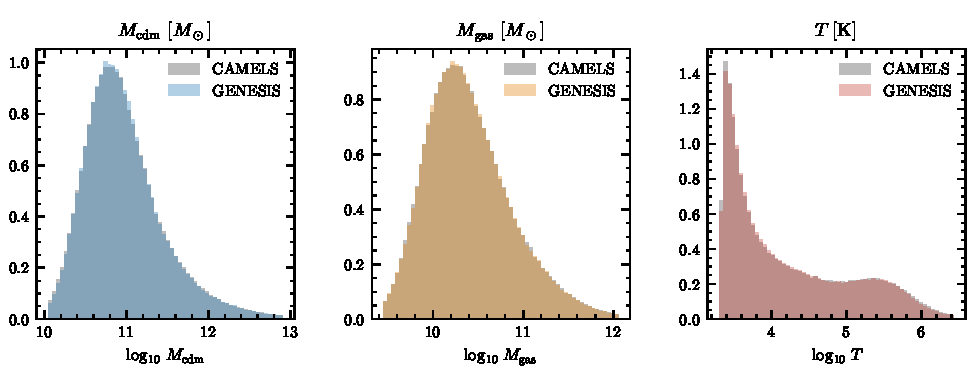
\includegraphics[width=\columnwidth]{figs/lh/lh_pixel_hist.pdf}
%   \inlinefigcaption{Per-channel LH pixel-value histograms in $\log_{10}$ space
%     ($N_{\rm sim}=100$, $n_{\rm gen}=30$ per sim).
%     Filled grey histograms show the pooled CAMELS pixel distribution;
%     coloured histograms show the \textsc{Genesis} ensemble.}
% \end{inlinefigure}

% Fig.~\ref{fig:figs5b} shows the per-simulation field mean on a
% simulation-by-simulation basis.
% Points lying close to the $y=x$ diagonal confirm that the
% \textsc{Genesis} ensemble reproduces the mean field amplitude across
% the full LH parameter range.

% \begin{inlinefigure}{fig:figs5b}
%   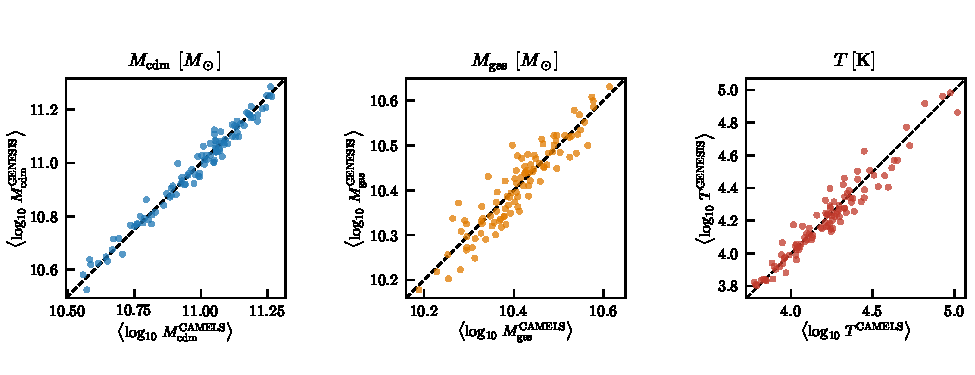
\includegraphics[width=\columnwidth]{figs/lh/lh_pixel_mean.pdf}
%   \inlinefigcaption{Per-simulation field mean on the LH test set
%     ($N_{\rm sim}=100$, $n_{\rm gen}=30$ per sim).
%     Horizontal axis: CAMELS simulation mean; vertical axis: mean of the
%     \textsc{Genesis} ensemble generated at the same conditioning vector.
%     The dashed line marks $y=x$.}
% \end{inlinefigure}

% \section{Swin Transformer comparison}  % TODO: Swin 실험 결과 추가 후 주석 해제
% \label{app:swin}
%
% We compare the primary U-Net architecture against a Swin Transformer
% \citep{Liu2021} backbone of comparable parameter count.
% The Swin variant uses the same OT flow-matching objective, conditioning
% scheme, and training procedure as the U-Net, differing only in the
% backbone (shifted-window self-attention replacing the convolutional
% encoder--decoder).
% Table~\ref{tab:swin_comparison} summarizes the key evaluation metrics
% for both architectures.
% The U-Net achieves lower cross-power residuals for the
% feedback-sensitive pairs ($\Mcdm$--$\Tgas$ and $\Mgas$--$\Tgas$),
% consistent with the hypothesis that circular convolution provides a
% more natural inductive bias for periodic-boundary fields.
% The Swin variant shows higher inference latency due to the cost of
% shifted-window attention at multiple scales.
%
% \begin{table*}
%   \centering
%   \small
%   \setlength{\tabcolsep}{6pt}
%   \begin{tabular}{lcccc}
%     \hline
%     Metric & U-Net & Swin-B & Swin-L & Pass thr. \\
%     \hline
%     ...
%   \end{tabular}
%   \label{tab:swin_comparison}
% \end{table*}

\label{lastpage}
\end{document}
